\documentclass{article}
\usepackage{graphicx}

\title{Laporan Database 2}
\author{Putri Nella (1184017)}
\date{31 October 2019}

\begin{document}

\maketitle

\section{Langkah-Langkah Pembuatan Sistem Informasi di Oracle Apex:}
\begin{enumerate}
    \item Langkah pertama yaitu membuka link https://apex.oracle.com/en/.dan selanjutnya klik sign in.
  \begin{center}
    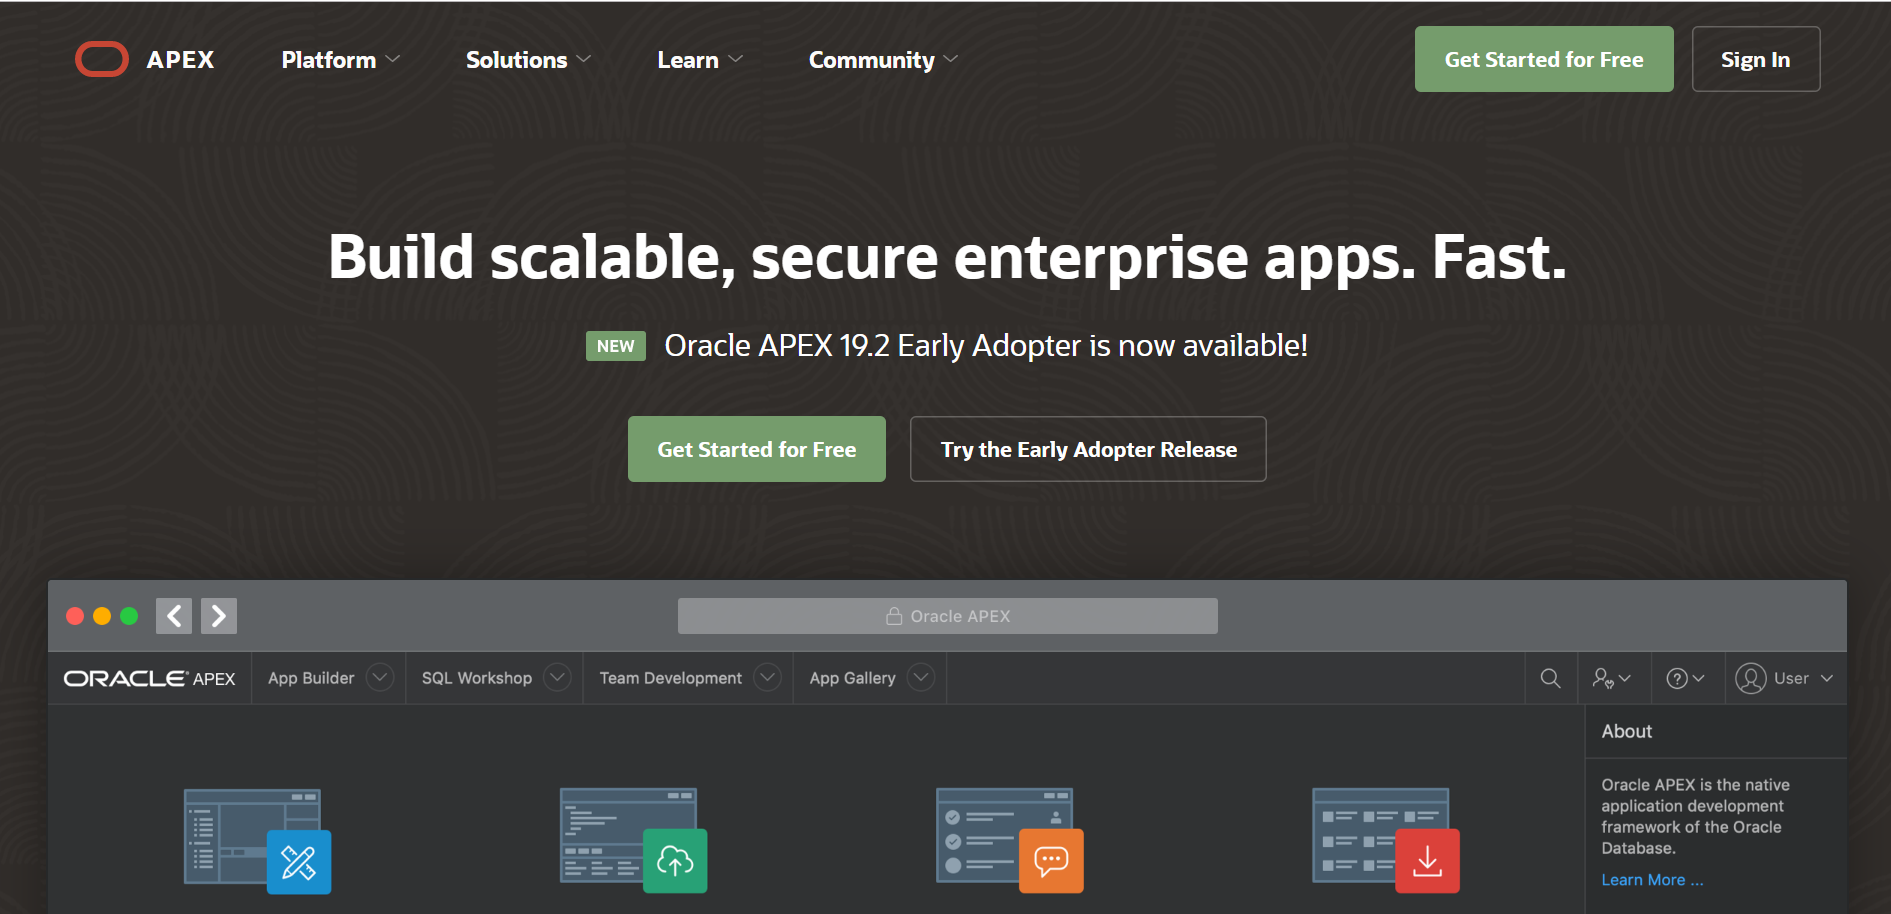
\includegraphics[width=.8\textwidth]{figure/1.PNG}
\end{center}
    \item isi data kita.. seperti dibawa ini.
    \begin{center}
    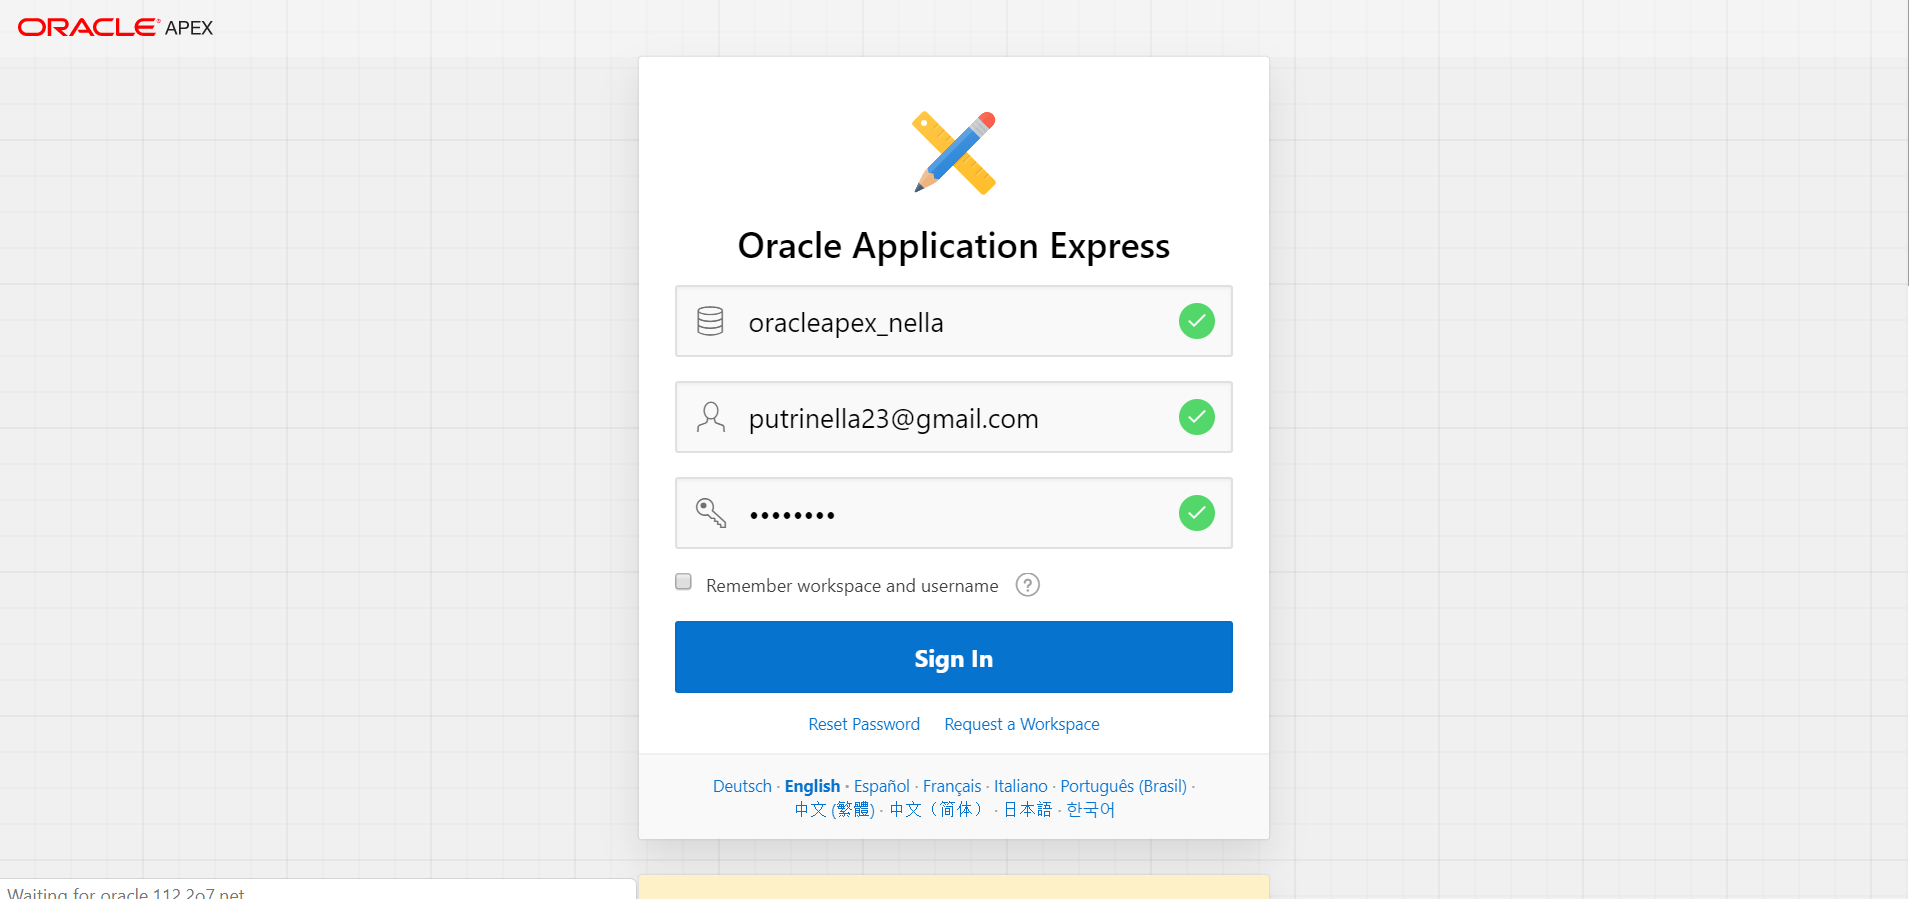
\includegraphics[width=.8\textwidth]{figure/2.PNG}
\end{center}
    \item Untuk membuat aplikasi kita pilih app builder
    \begin{center}
    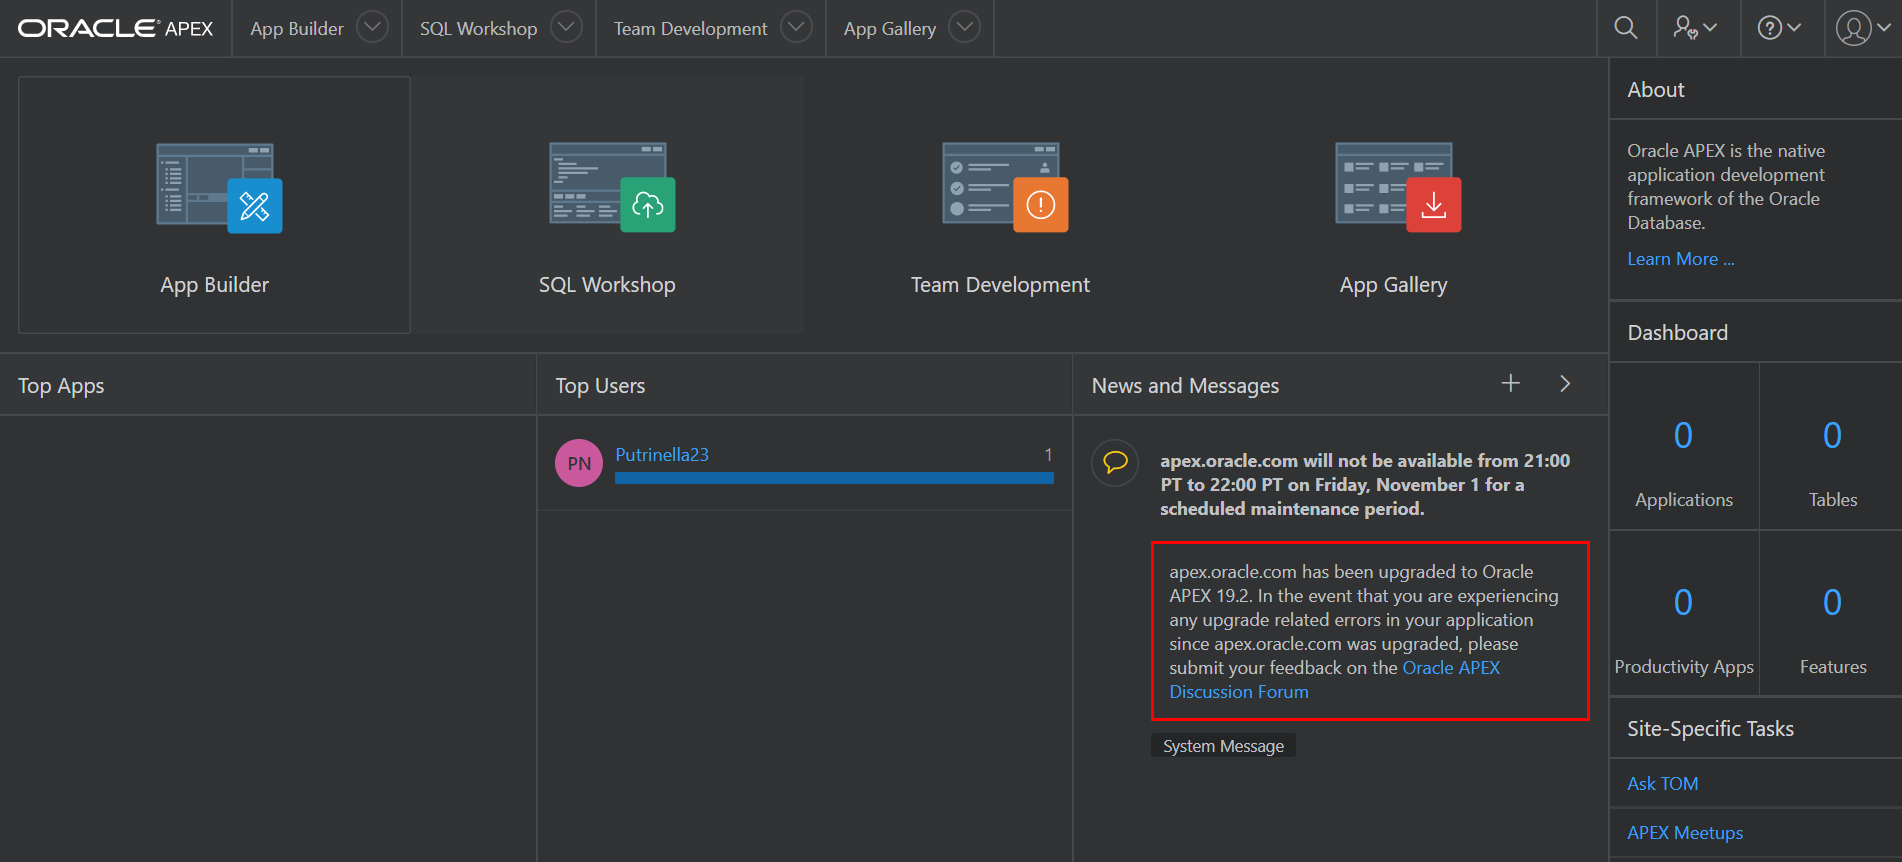
\includegraphics[width=.8\textwidth]{figure/3.PNG}
\end{center}
    \item Untuk memasukkan data dari komputer kita,kita pilih create.
    \begin{center}
    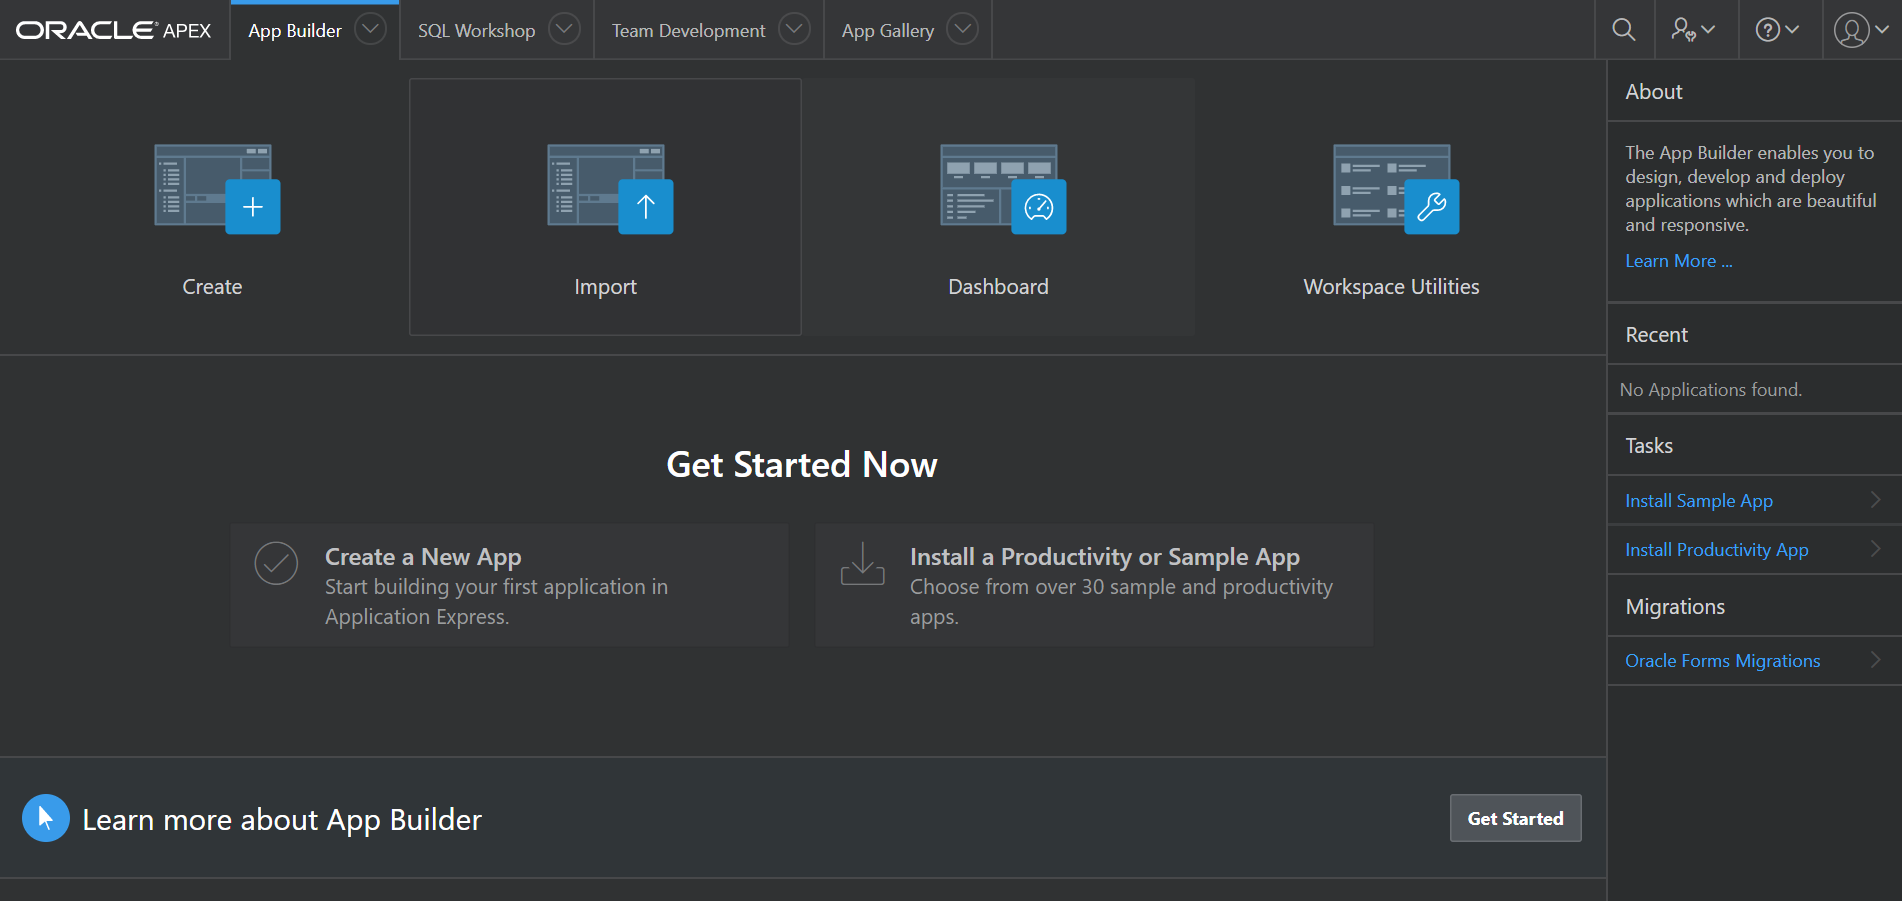
\includegraphics[width=.8\textwidth]{figure/4.PNG}
\end{center}
    \item untuk memasukkan data kita pilih From a file ,jika sudah kita pilih data mahasiswa yang ingin dimasukkan.
    \begin{center}
    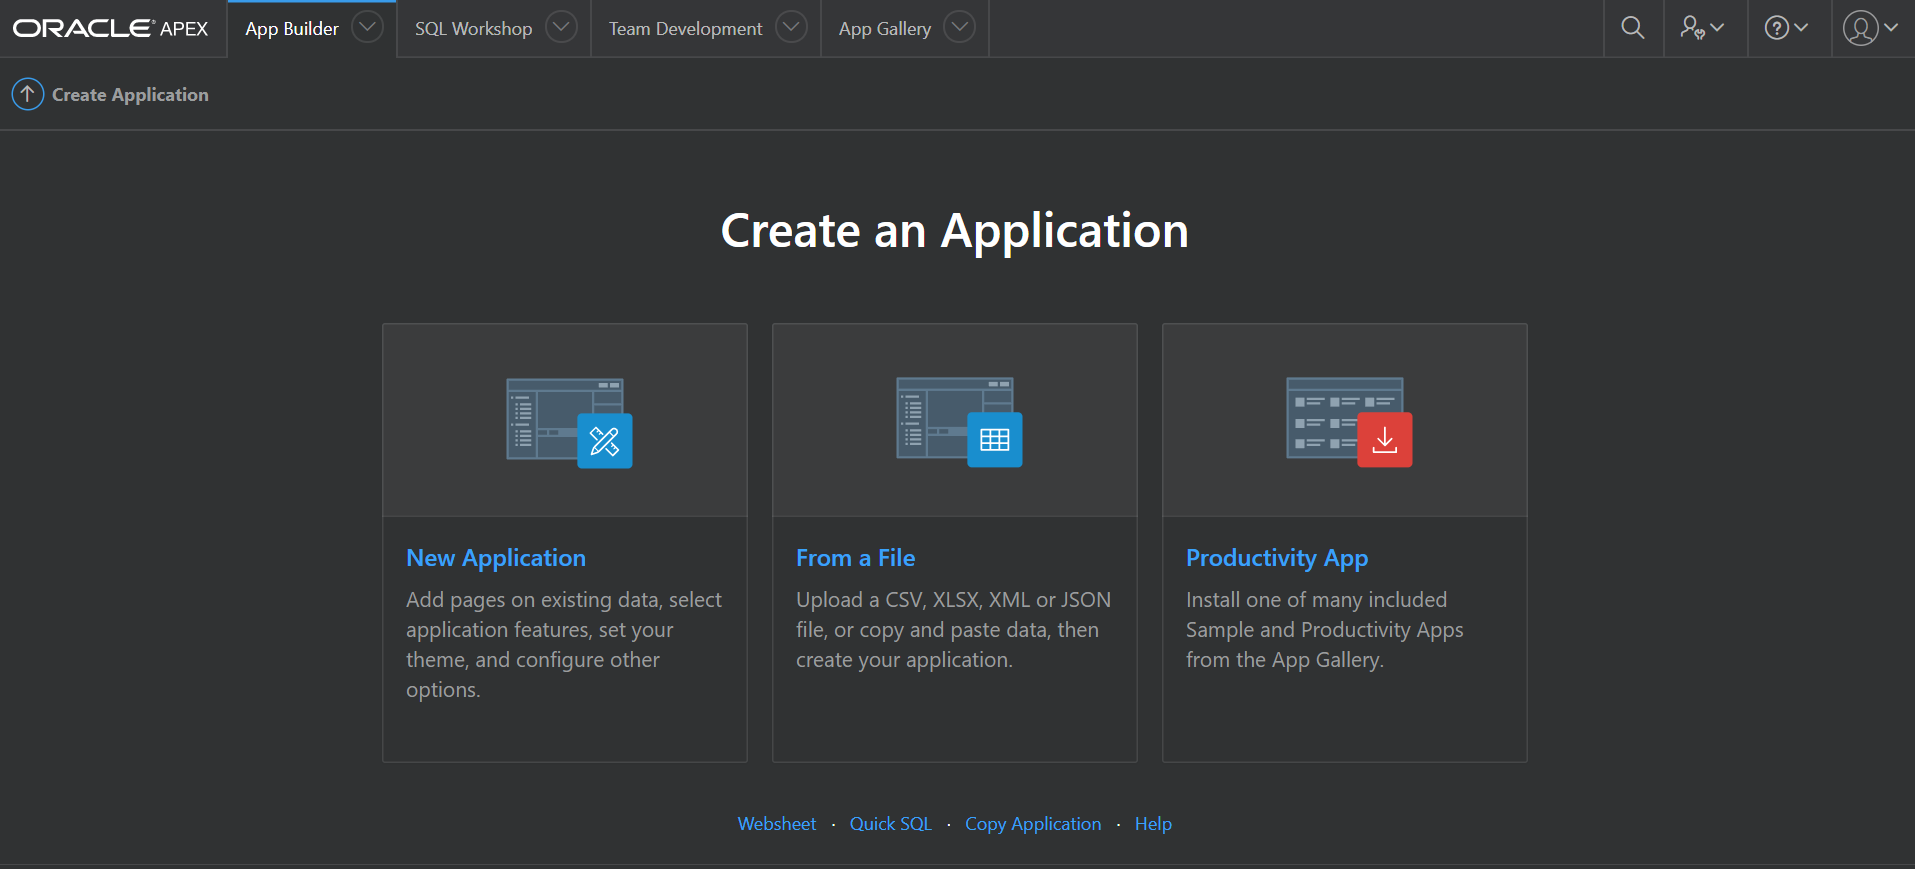
\includegraphics[width=.8\textwidth]{figure/5.PNG}
\end{center}
     \begin{center}
    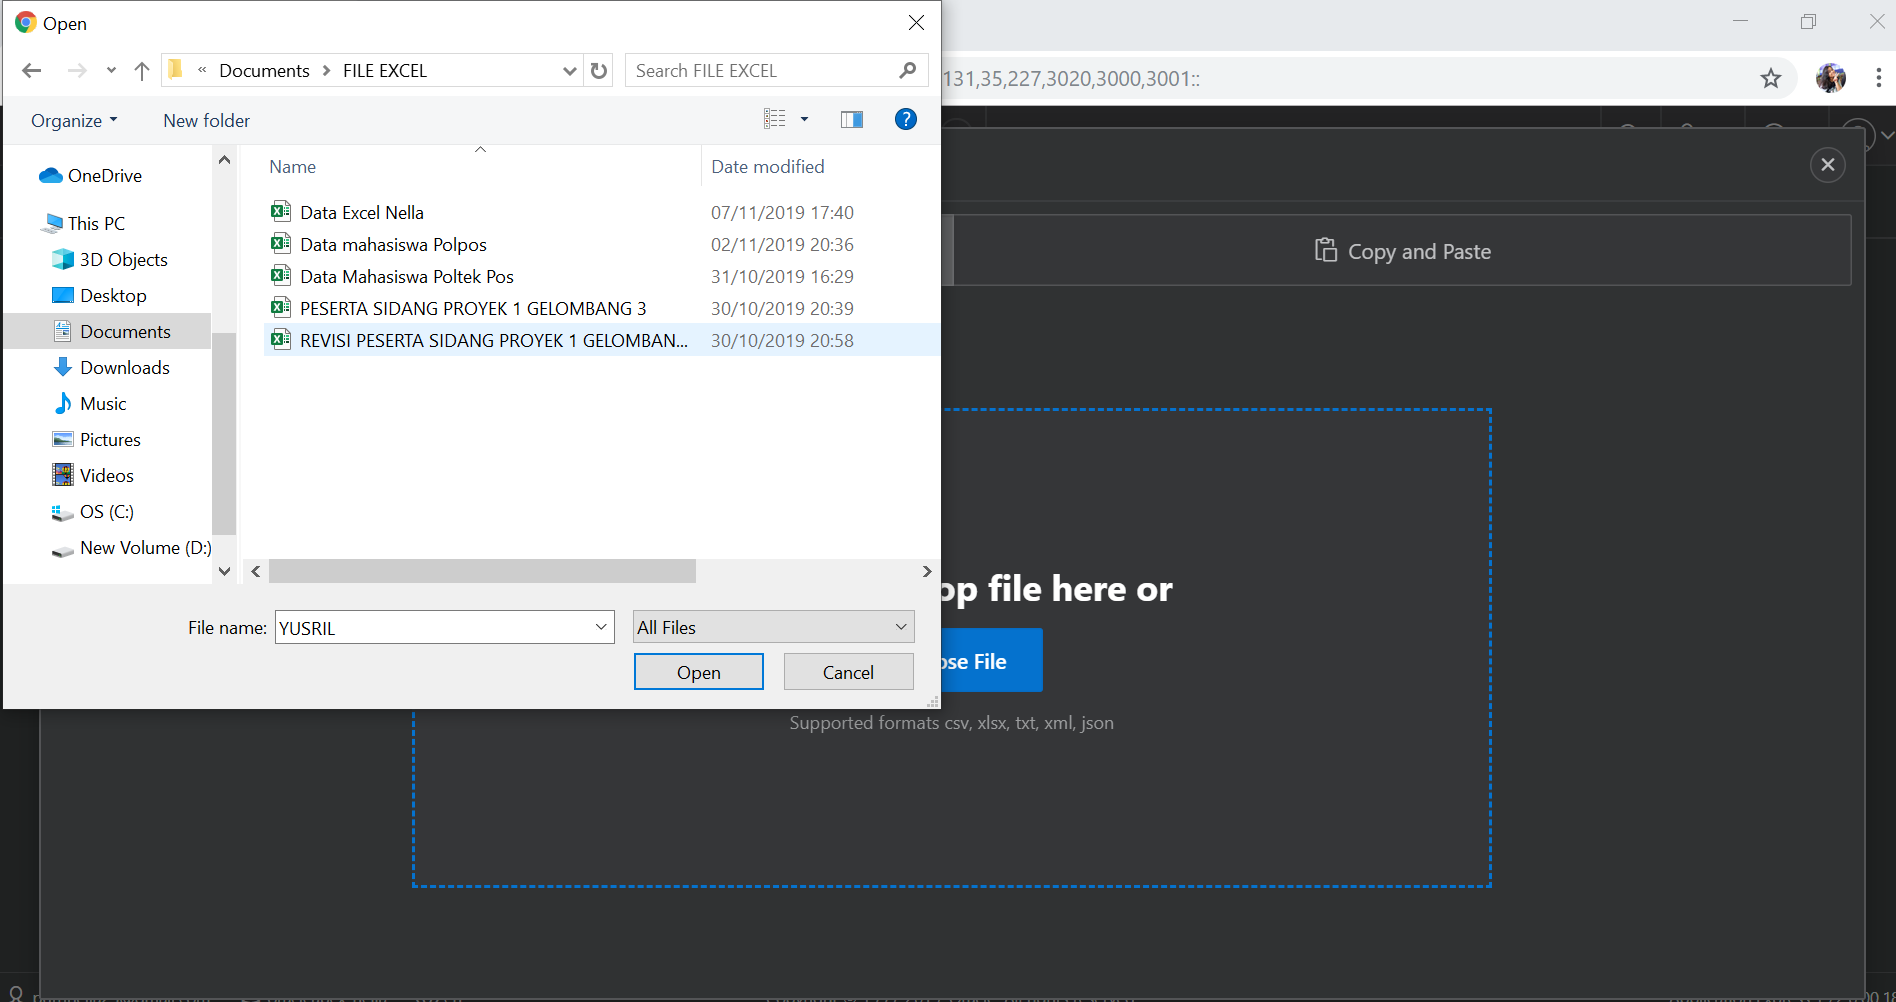
\includegraphics[width=.8\textwidth]{figure/18.PNG}
\end{center}
    \item Jika data telah berhasil di input maka akan tampil seperti ini..
    \begin{center}
    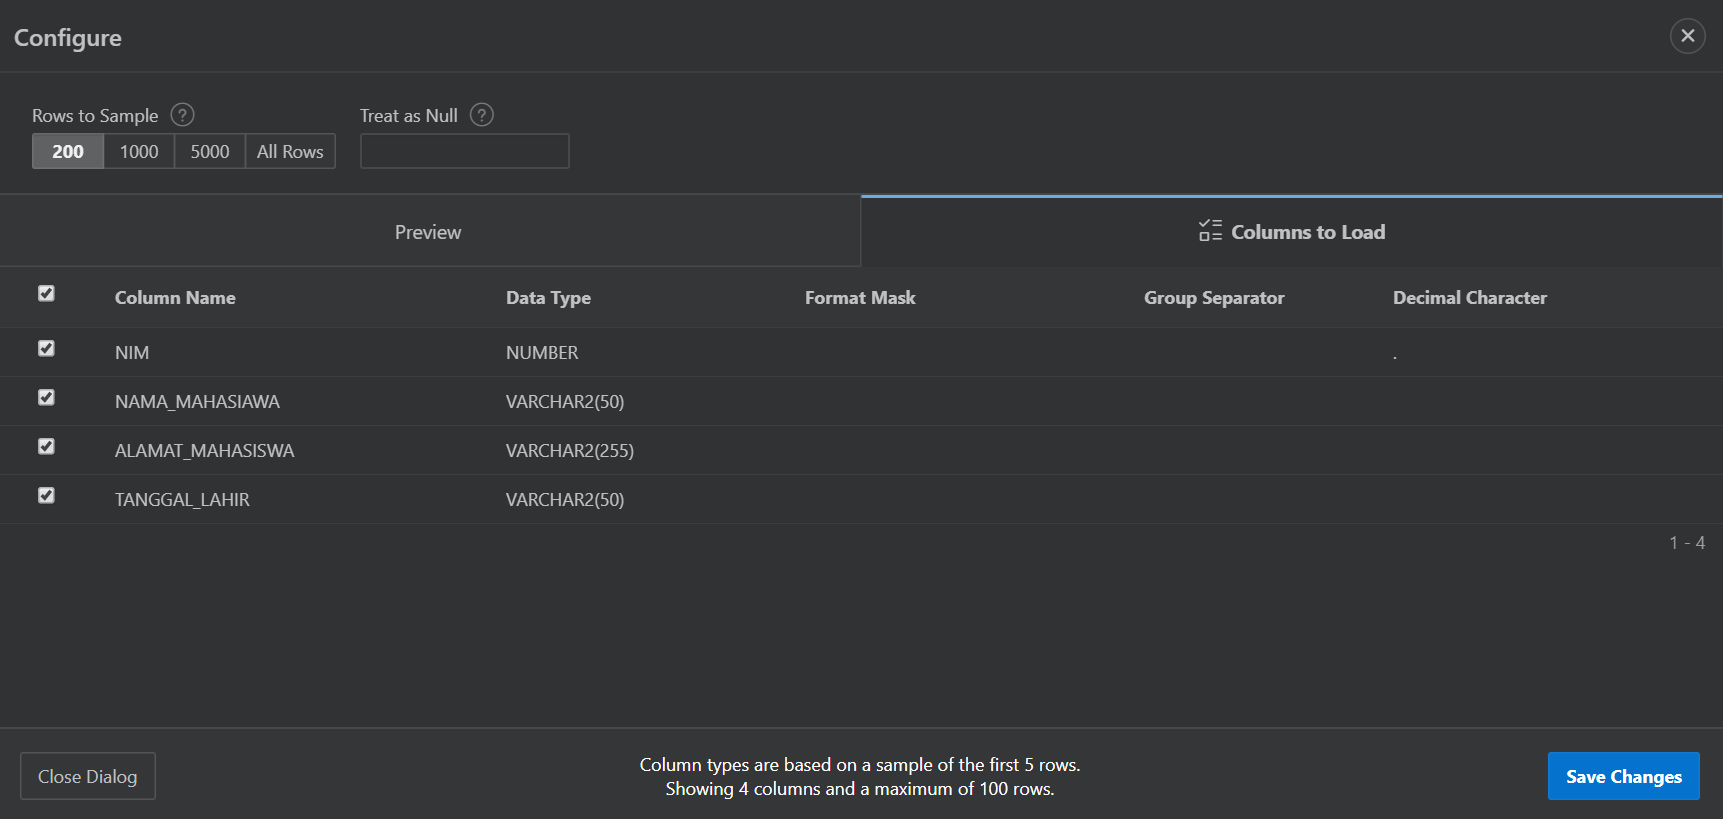
\includegraphics[width=.8\textwidth]{figure/20.PNG}
\end{center}
\item setelah itu isi nama table pada form yg telah tersedia,jika sudah selesai klik load data.
\begin{center}
    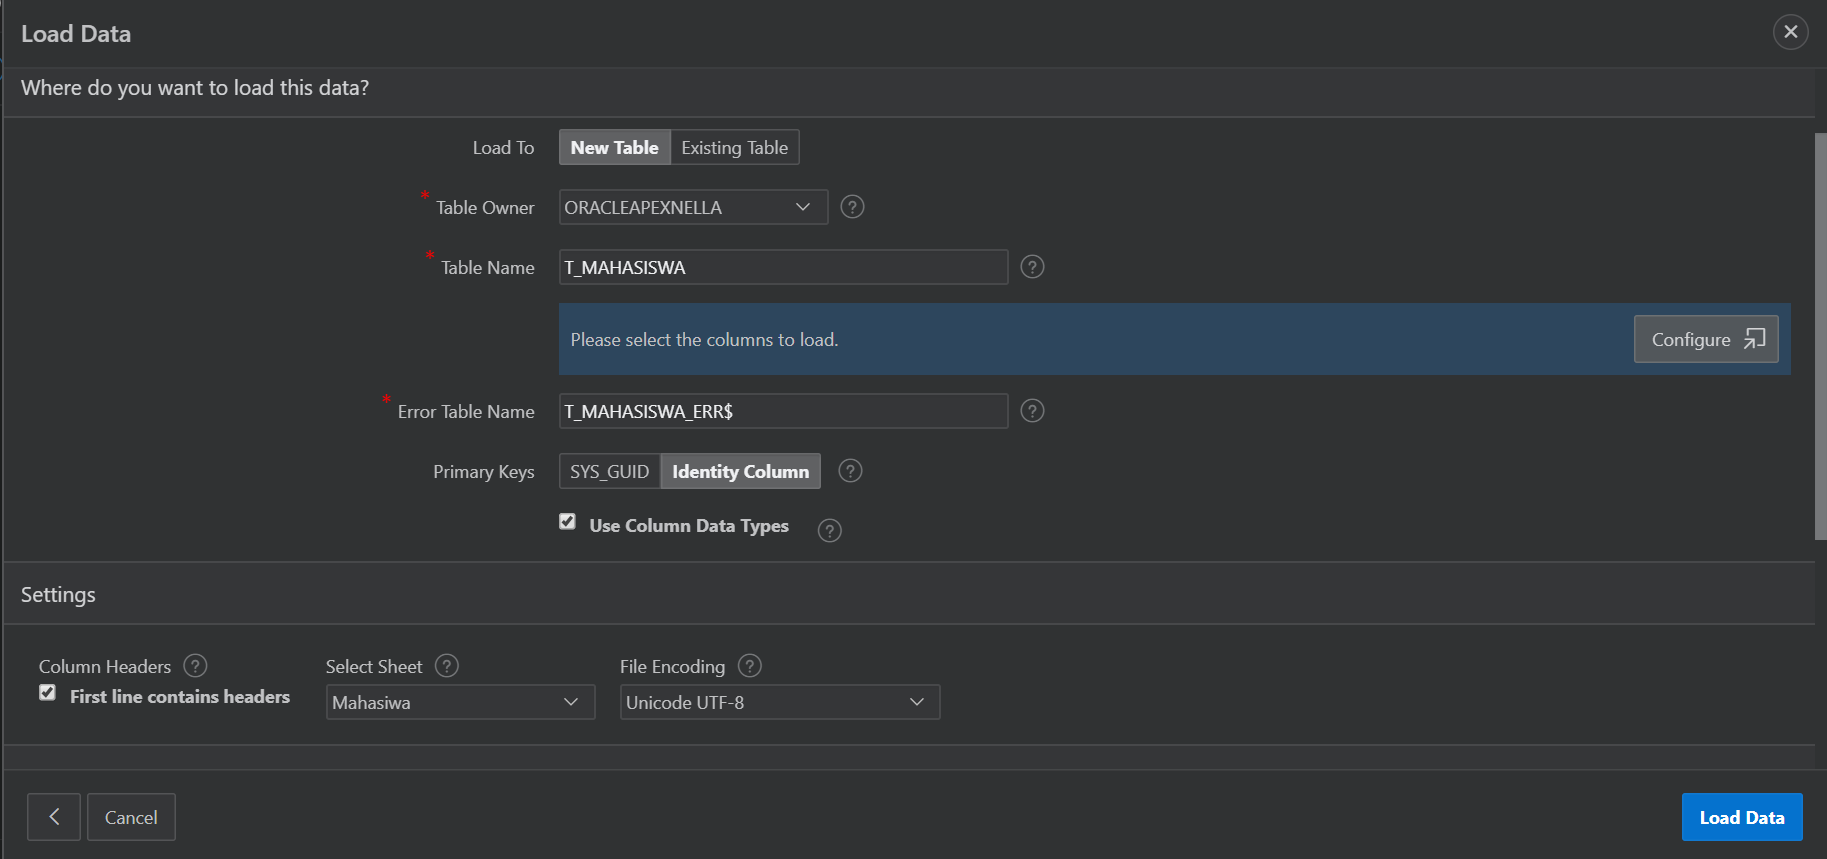
\includegraphics[width=.8\textwidth]{figure/9.PNG}
\end{center}
    \item jika telah selesai me load data maka akan dialihkan pada halaman dibawah ini .
    \begin{center}
    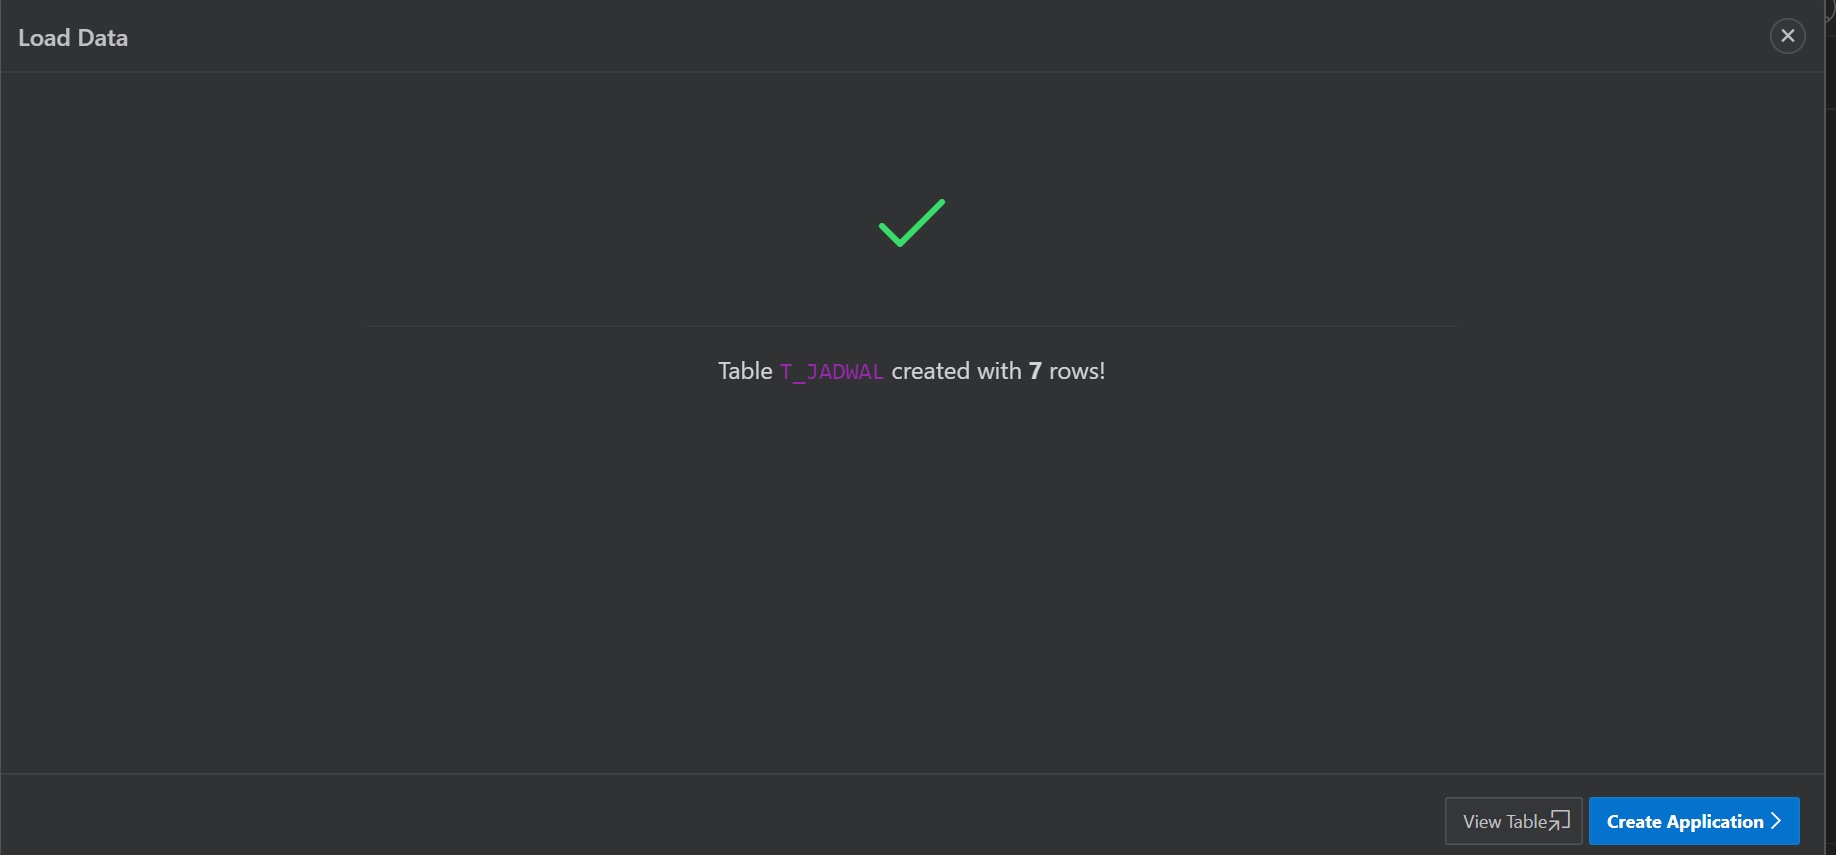
\includegraphics[width=.8\textwidth]{figure/12.PNG}
\end{center}
    \item lakukan cara diatas untuk menginput data dosen,kuliah,nilai,dan jadwal.
    \begin{center}
    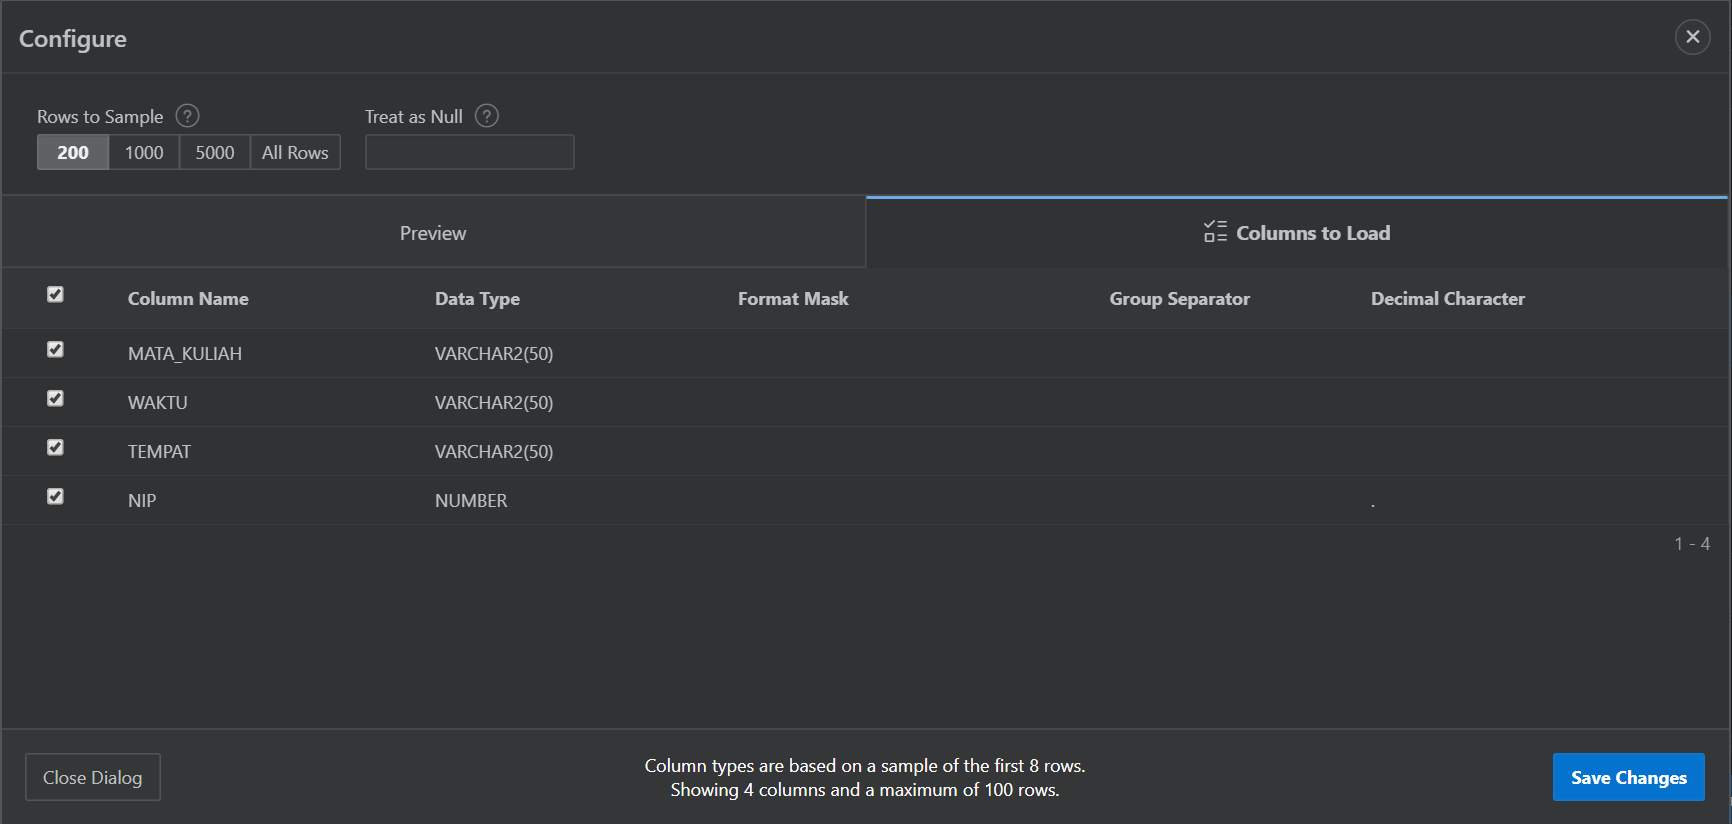
\includegraphics[width=.8\textwidth]{figure/19.PNG}
\end{center}
\begin{center}
    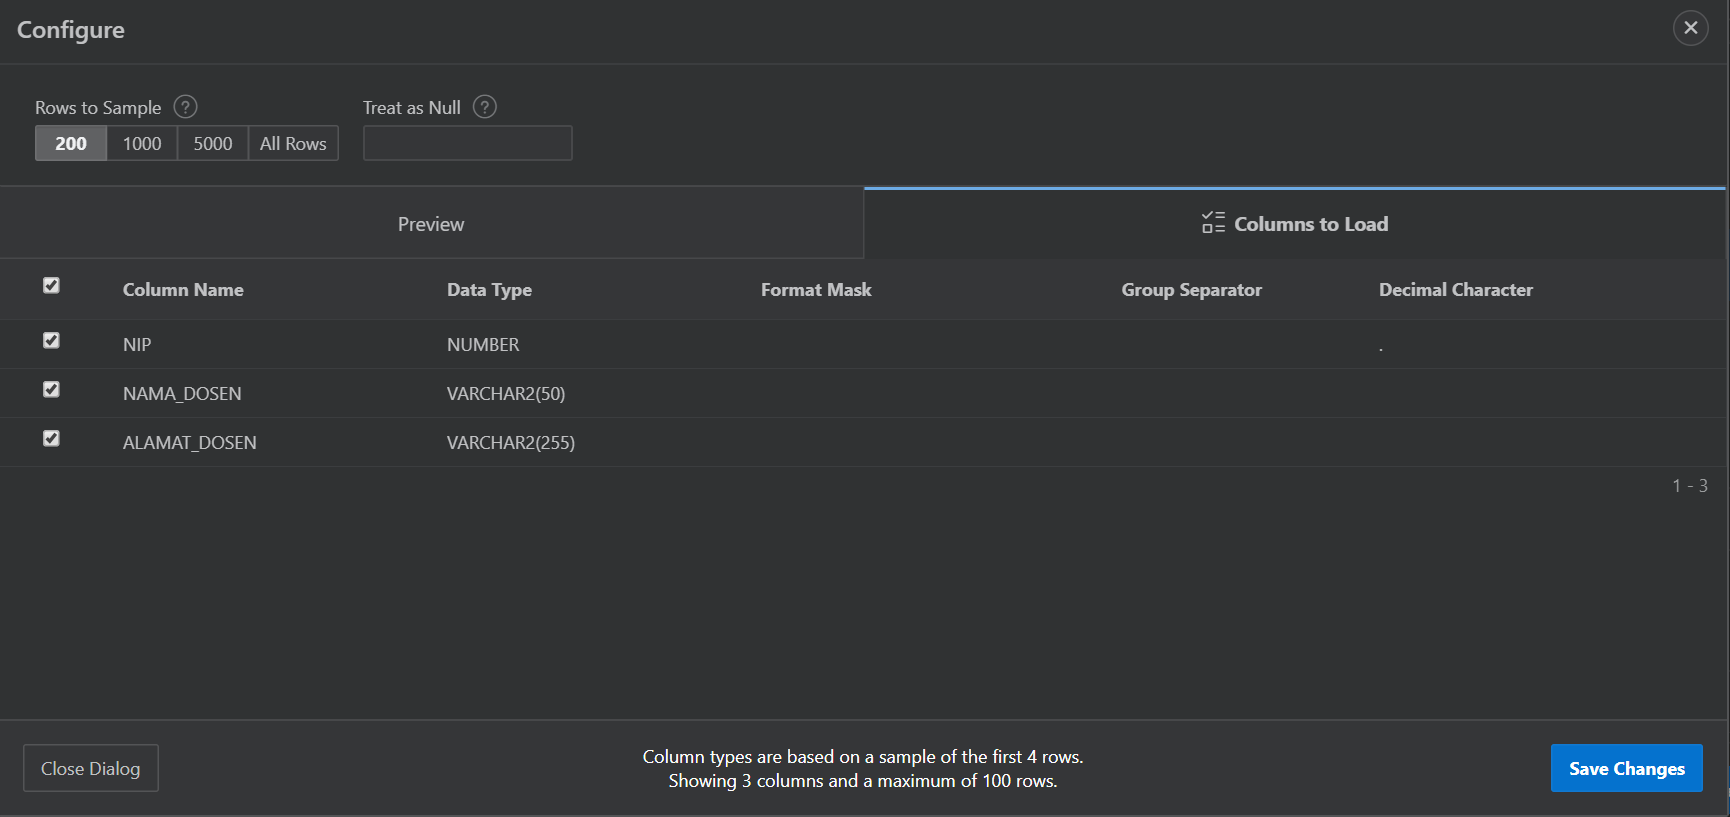
\includegraphics[width=.8\textwidth]{figure/21.PNG}
\end{center}
\begin{center}
    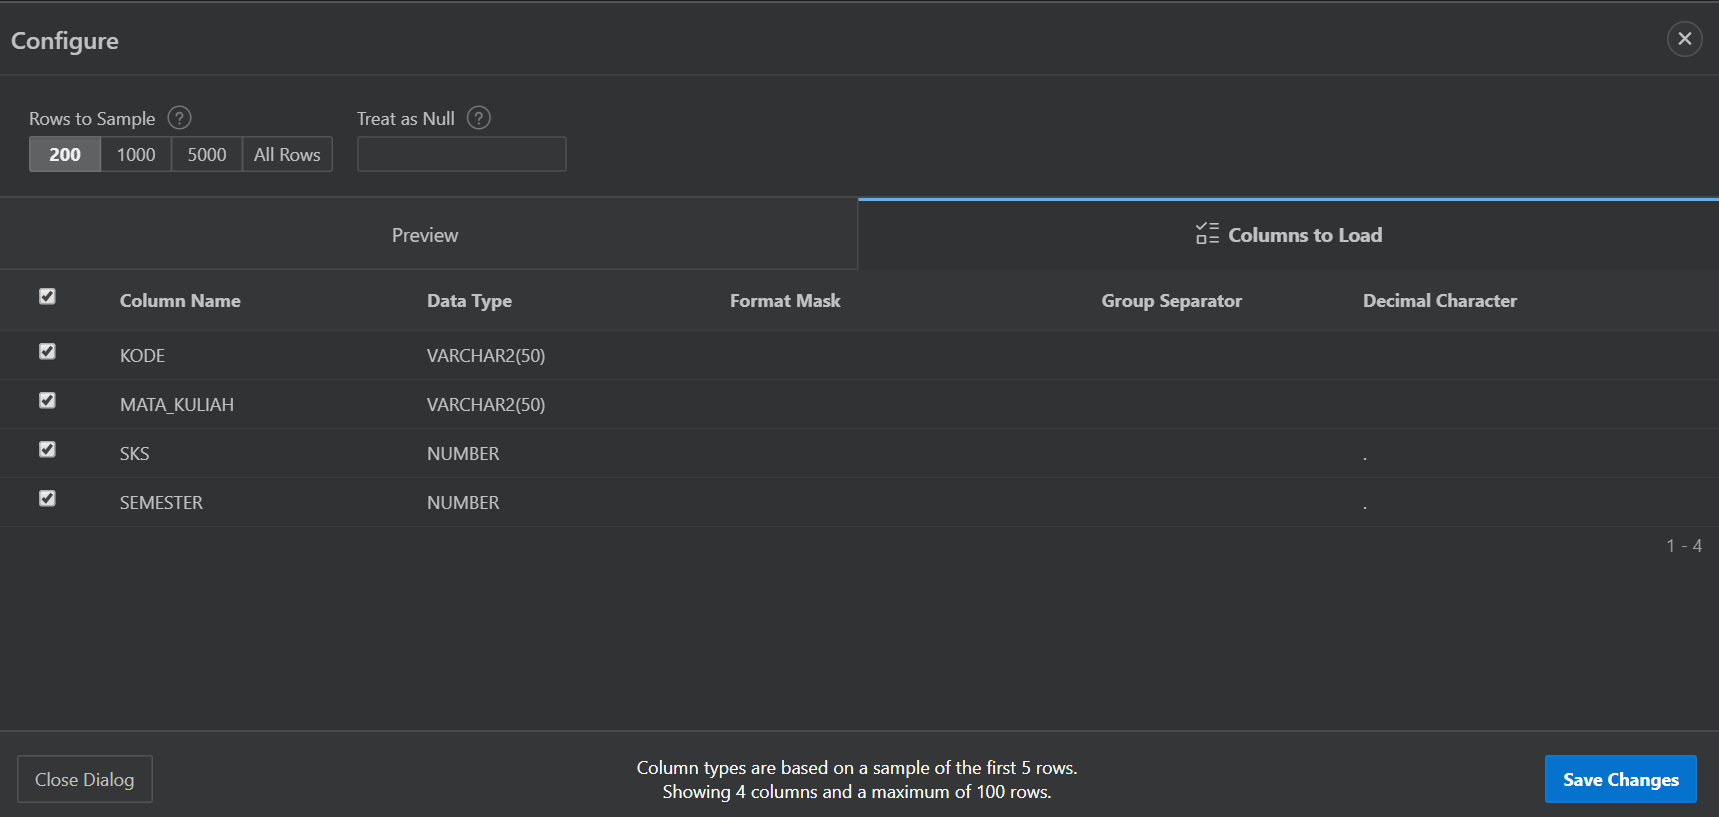
\includegraphics[width=.8\textwidth]{figure/22.PNG}
\end{center}
\begin{center}
    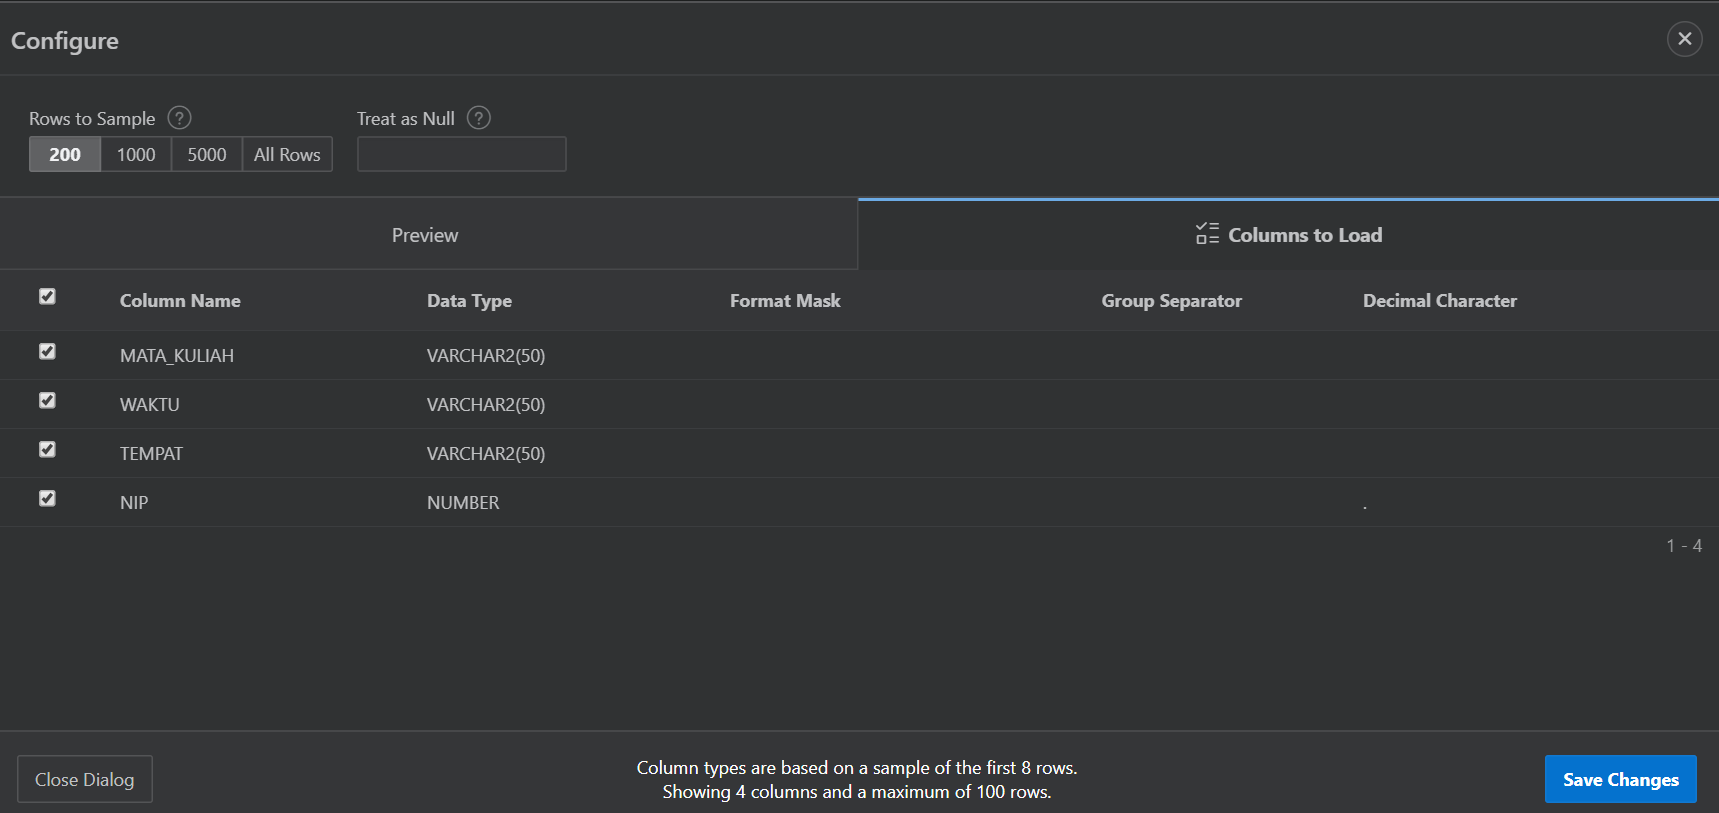
\includegraphics[width=.8\textwidth]{figure/23.PNG}
\end{center}
    \item jika data mahasiswa,dosen,nilai,kuliah,jadwal telah terinput dan belum mempunyai primary key,maka oracle apex akan secara otomatis menambahkannya,jadi kita buka object browser dan menghapus kolom id.
    \begin{center}
    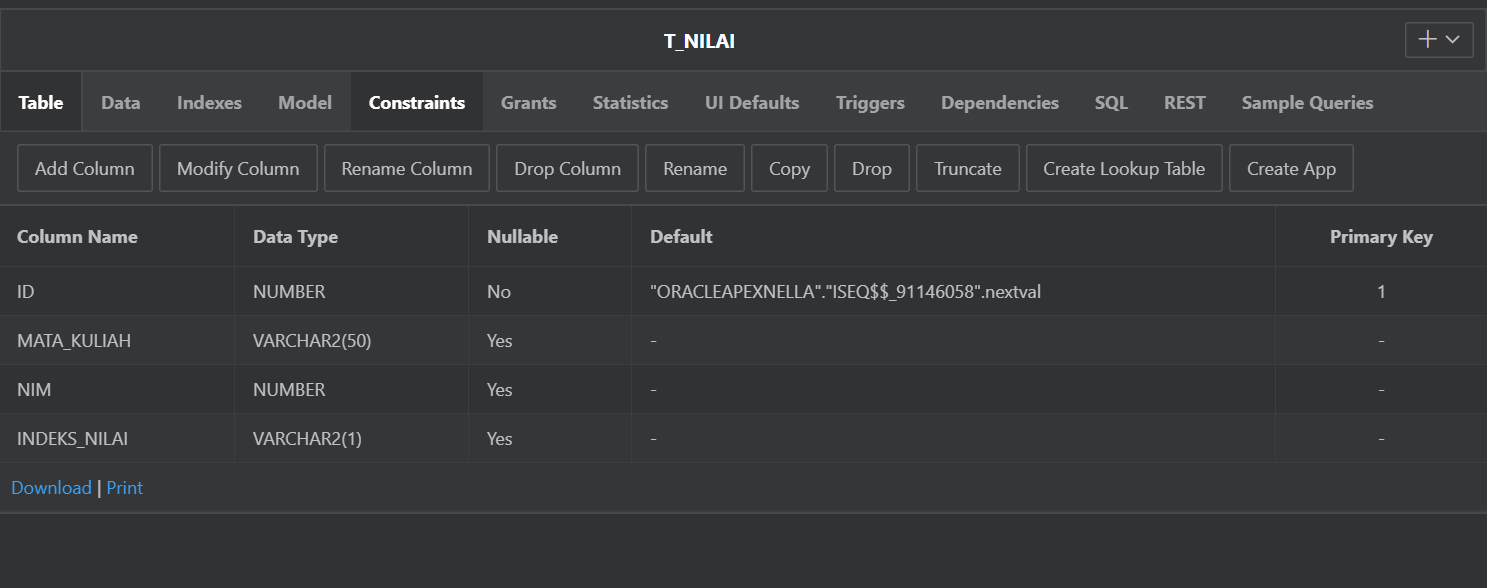
\includegraphics[width=.8\textwidth]{figure/13.PNG}
\end{center}
\begin{center}
    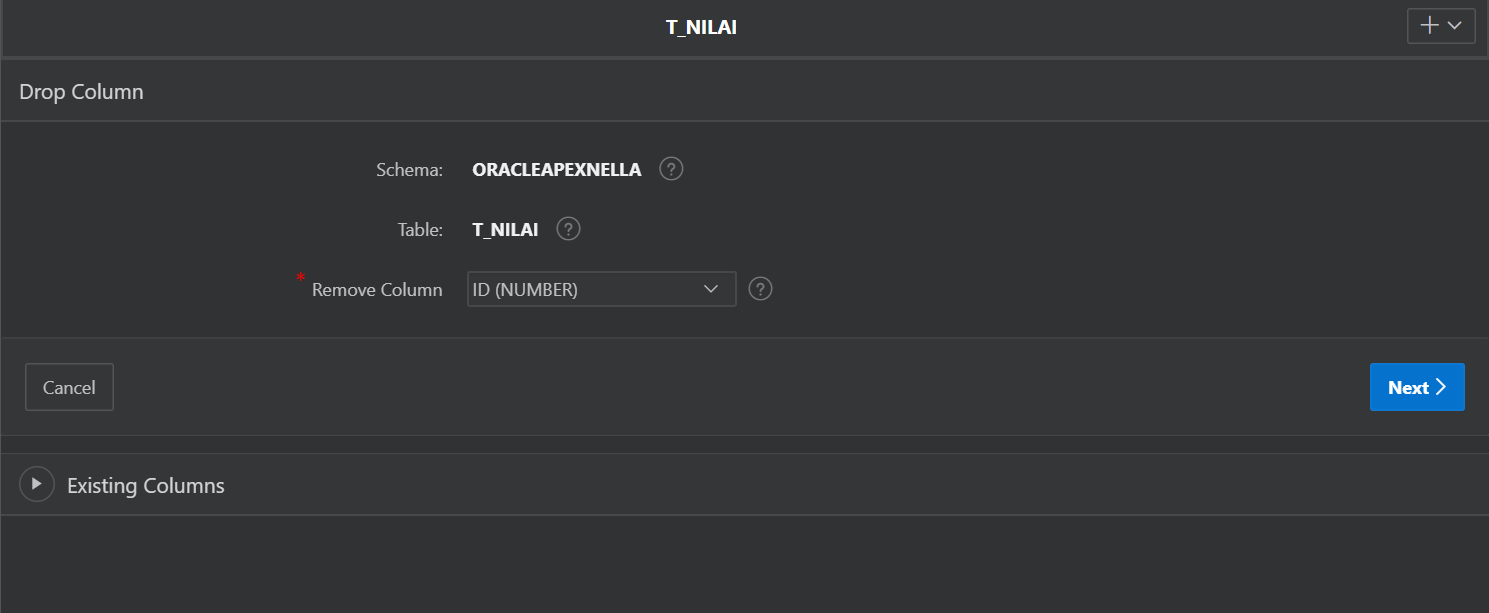
\includegraphics[width=.8\textwidth]{figure/14.PNG}
\end{center}
    \item Apabila id kolom telah terhapus,selanjutnya kita akan memasukkan id secara manual pada setiap table.
    \begin{center}
    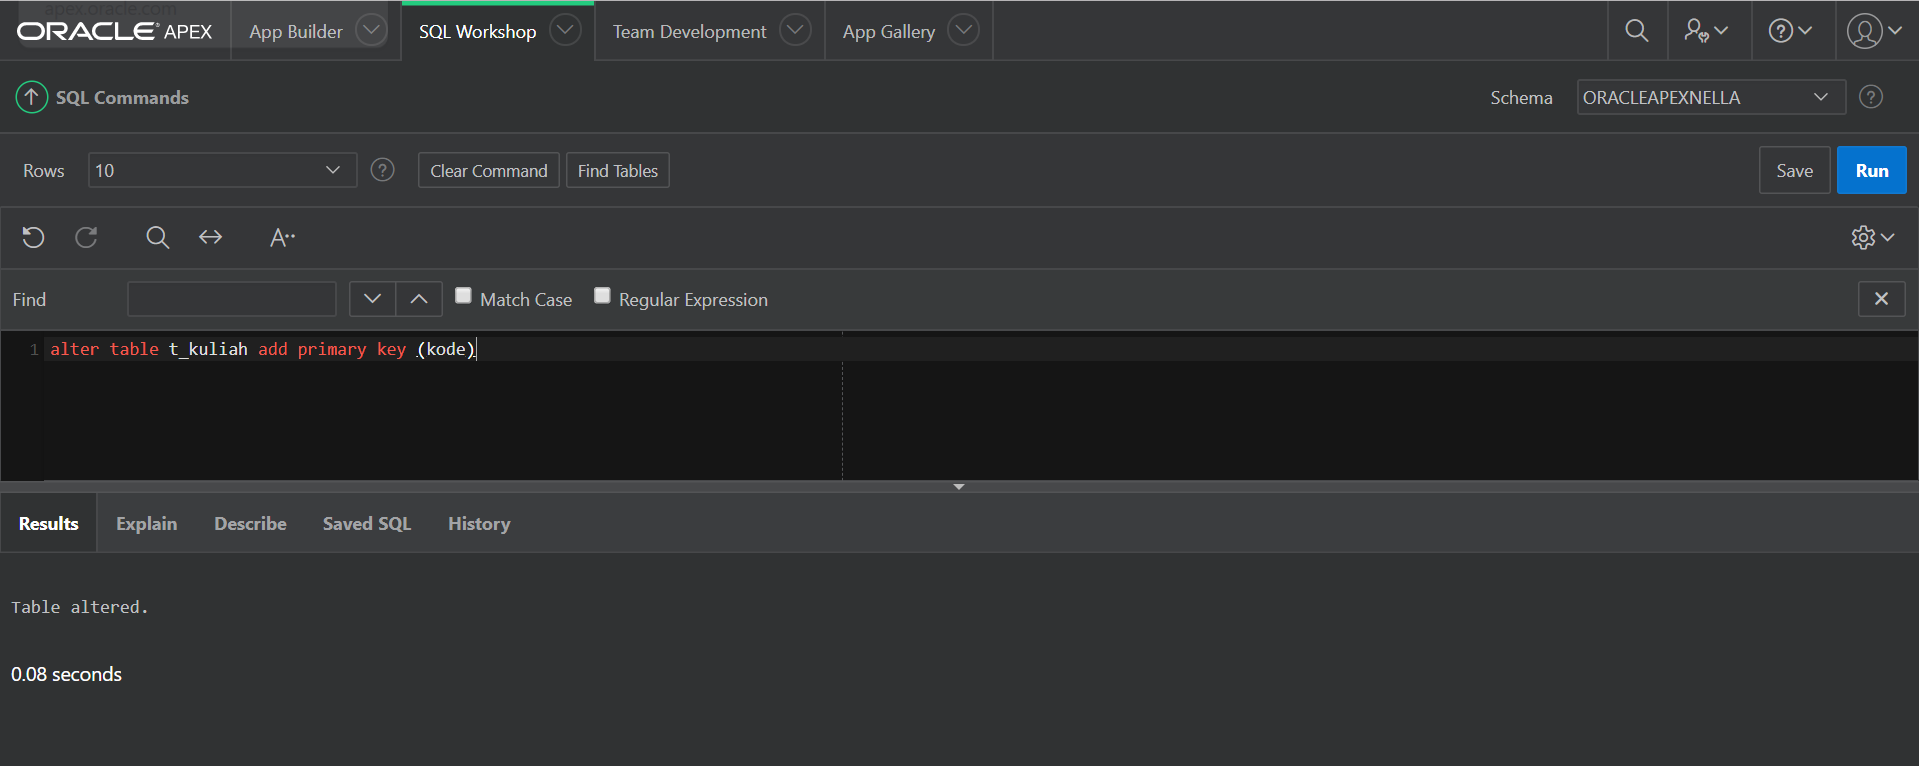
\includegraphics[width=.8\textwidth]{figure/17.PNG}
\end{center}
\begin{center}
    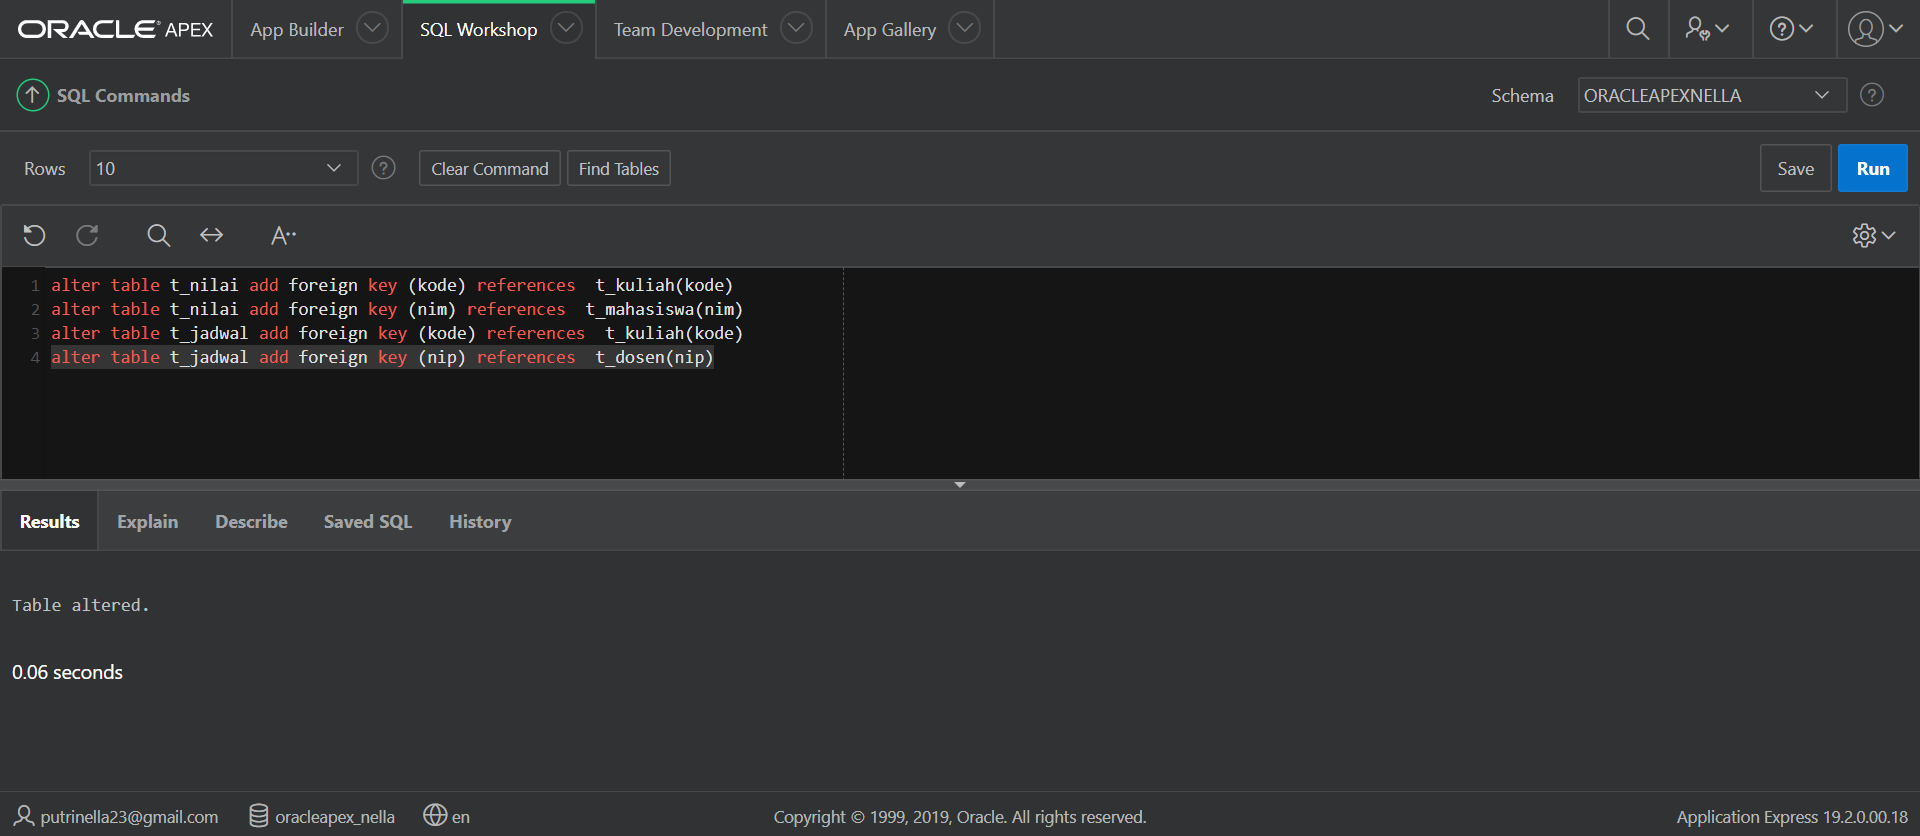
\includegraphics[width=.8\textwidth]{figure/25.PNG}
\end{center}
    \item apabila data telah ternomalisasi dengan benar maka kita dapat mengcreate application.
    \begin{center}
    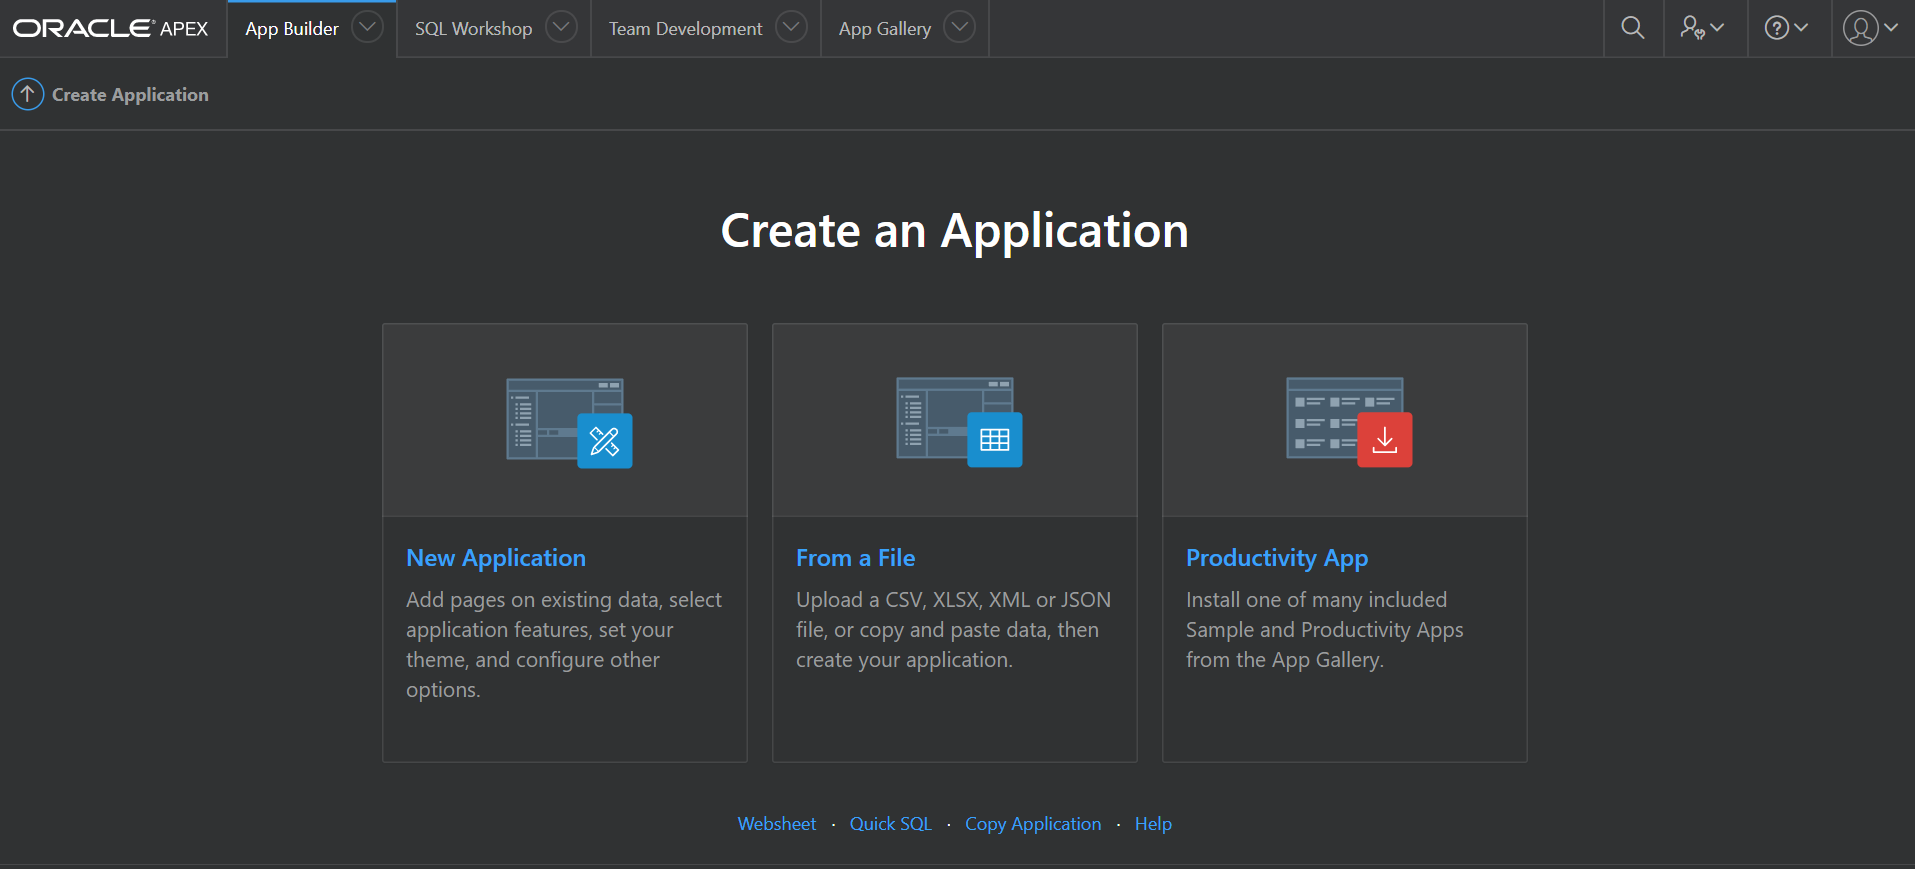
\includegraphics[width=.8\textwidth]{figure/5.PNG}
\end{center}
    \item jika telah tercreate maka akan muncul halaman seperti dibawaw ini.lali kita mengisi form name dengan nama aplikasi kita.
\begin{center}
    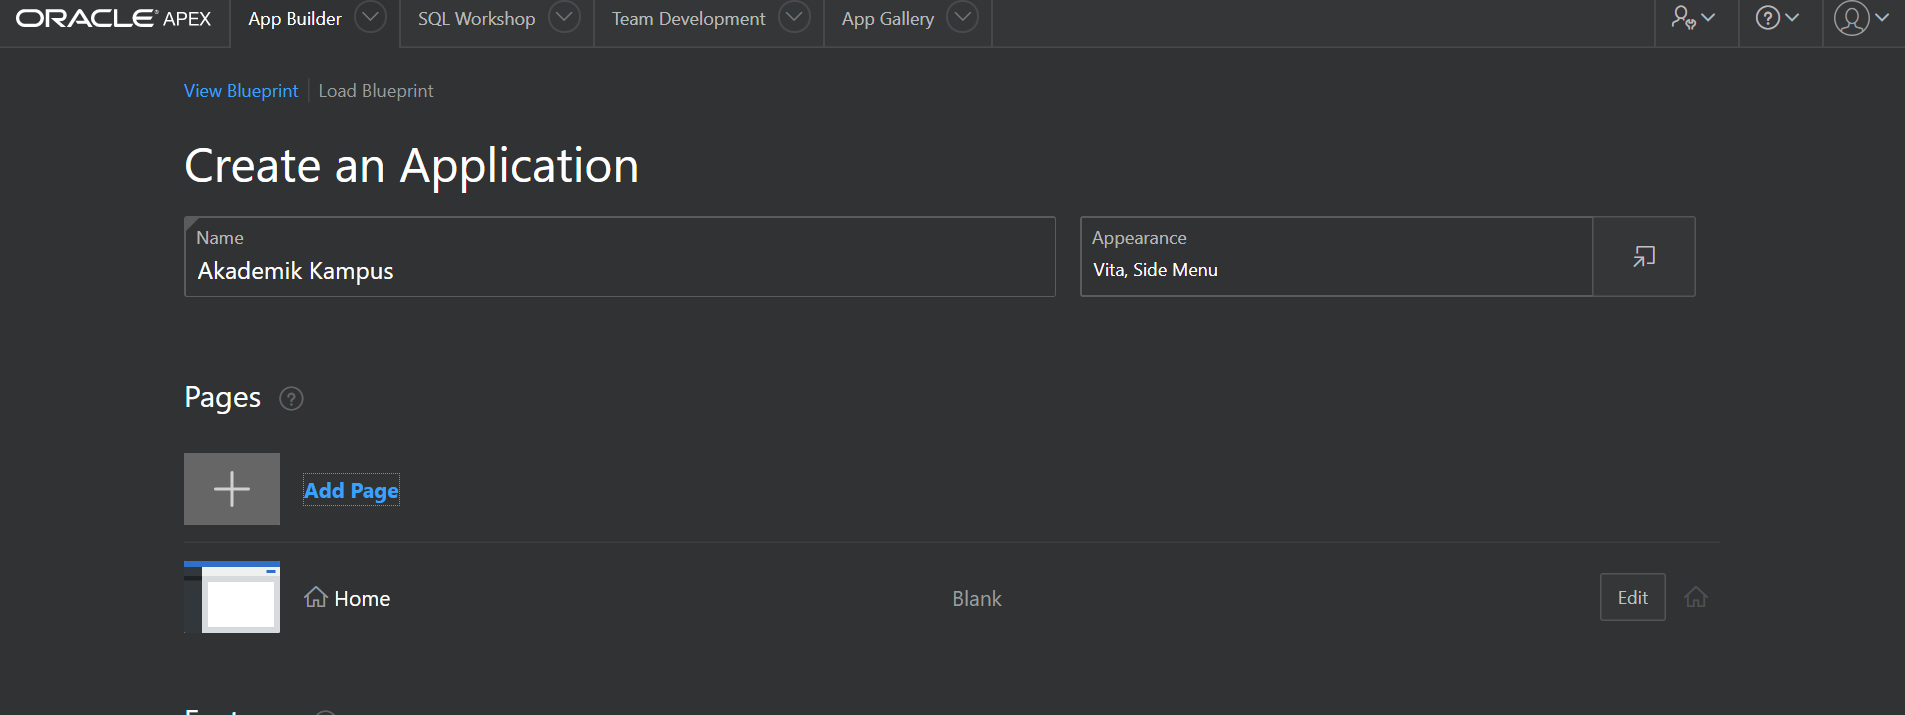
\includegraphics[width=.8\textwidth]{figure/26.PNG}
\end{center}
    \item Jika telah mengisi kita pilih page,dan setiap page kita beri nama yang berbeda dan masing-masing memasukkan datanya.
    \begin{center}
    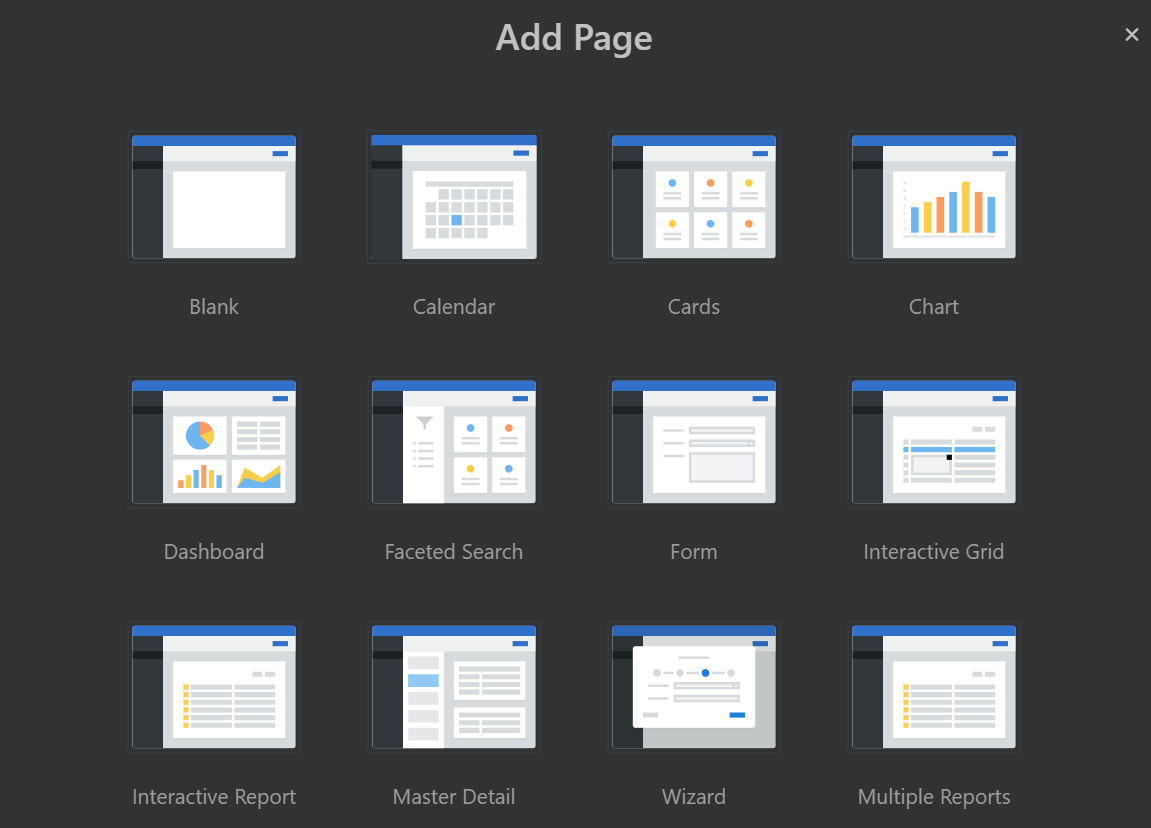
\includegraphics[width=.8\textwidth]{figure/27.PNG}
\end{center}
\begin{center}
    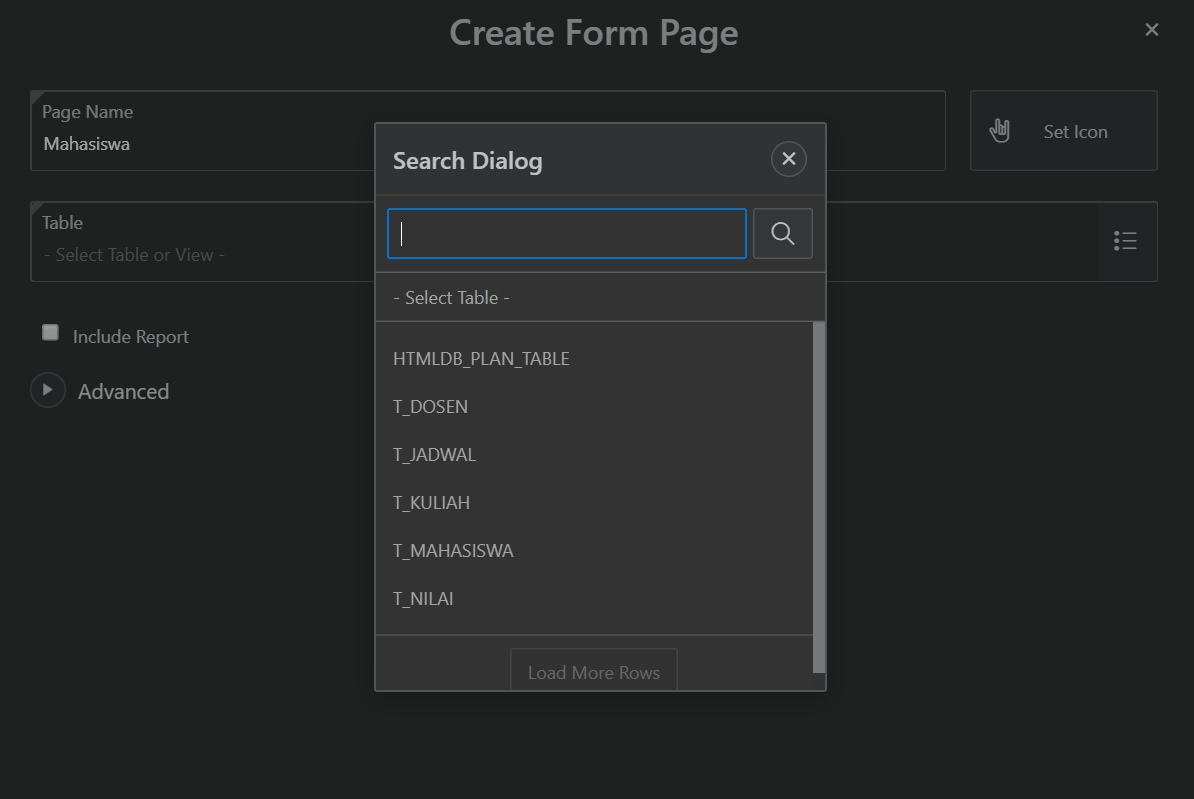
\includegraphics[width=.8\textwidth]{figure/28.PNG}
\end{center}
\begin{center}
    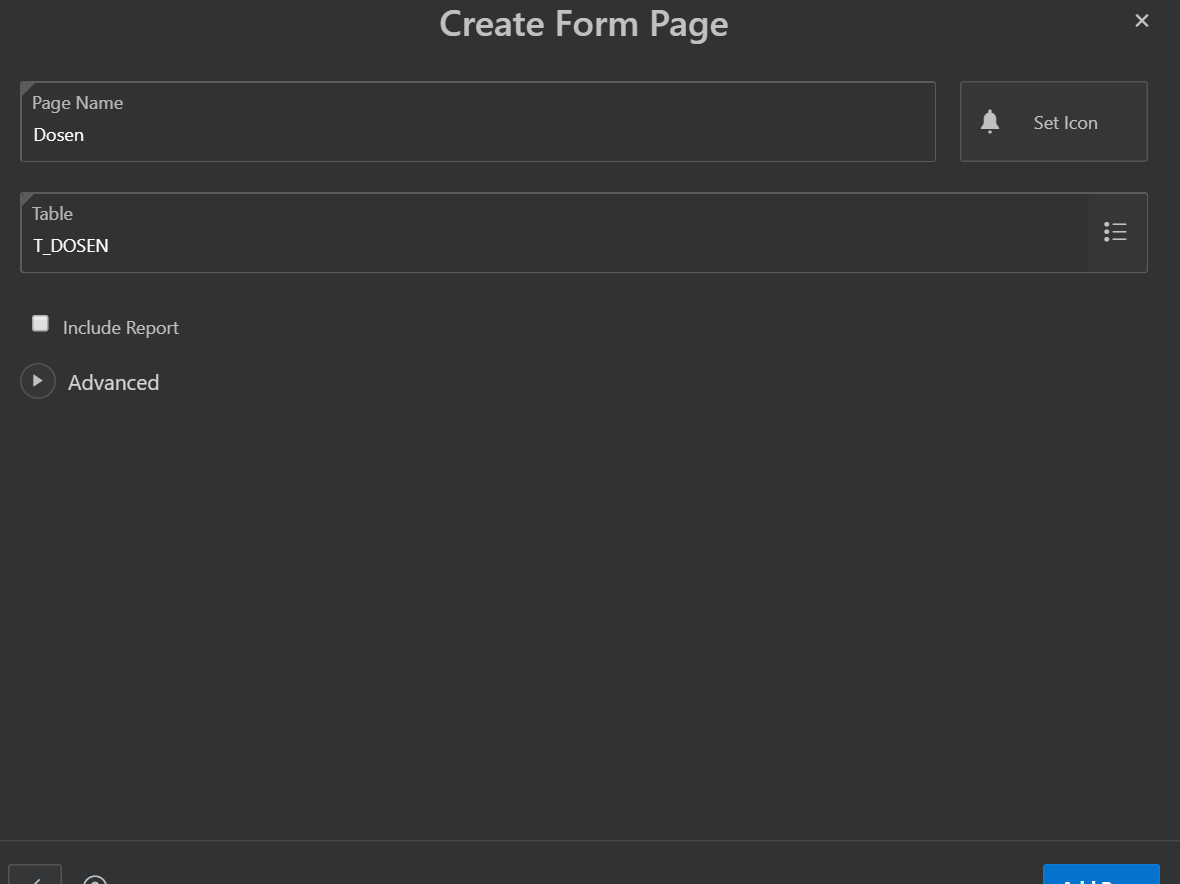
\includegraphics[width=.8\textwidth]{figure/29.PNG}
\end{center}
\begin{center}
    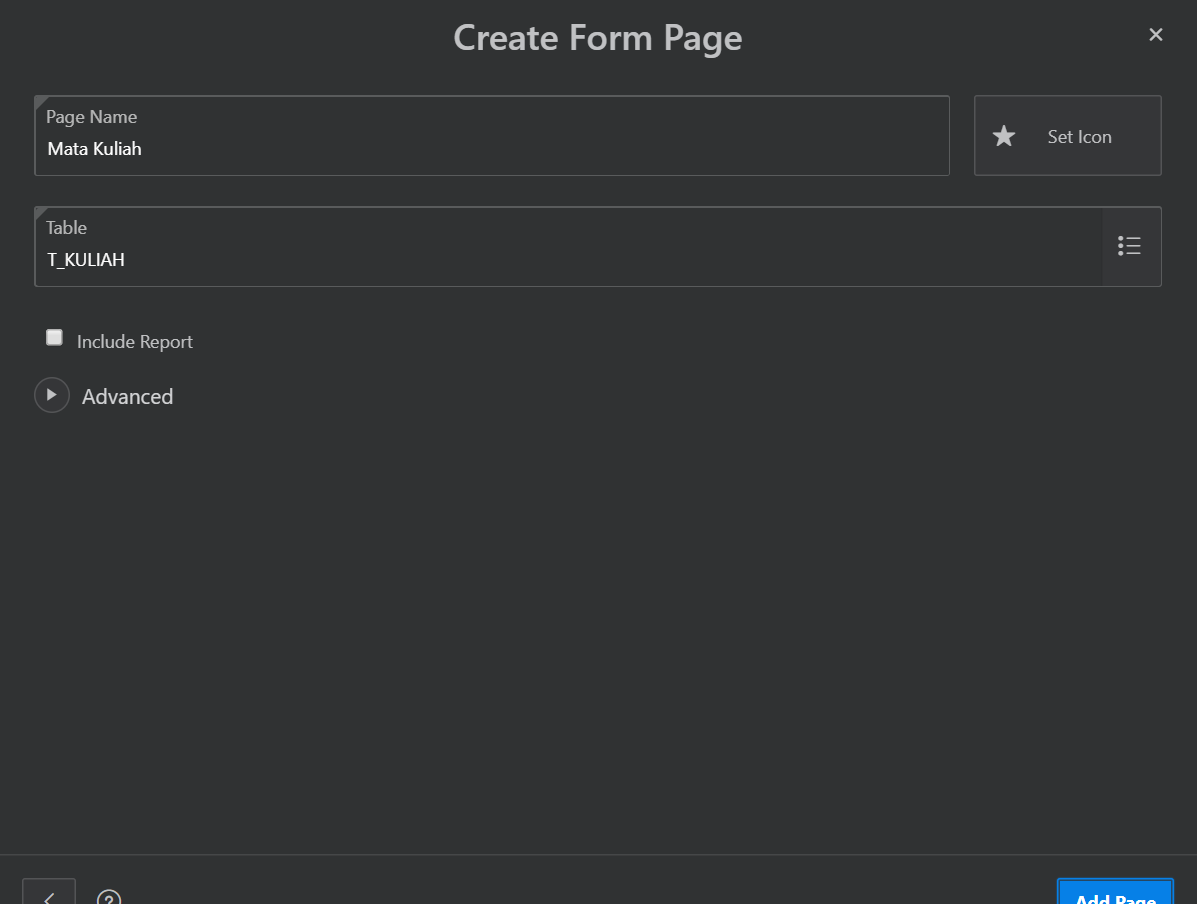
\includegraphics[width=.8\textwidth]{figure/30.PNG}
\end{center}
\begin{center}
    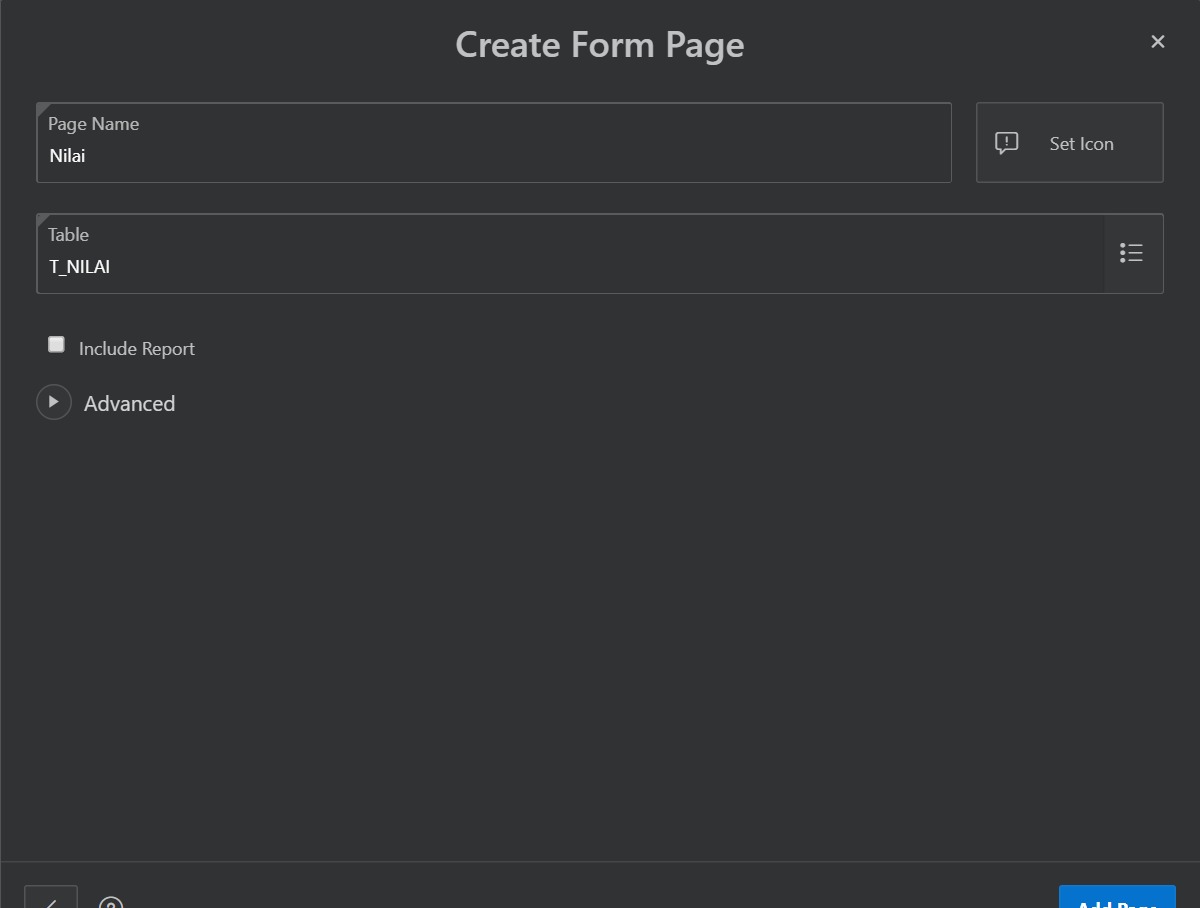
\includegraphics[width=.8\textwidth]{figure/31.PNG}
\end{center}
\begin{center}
    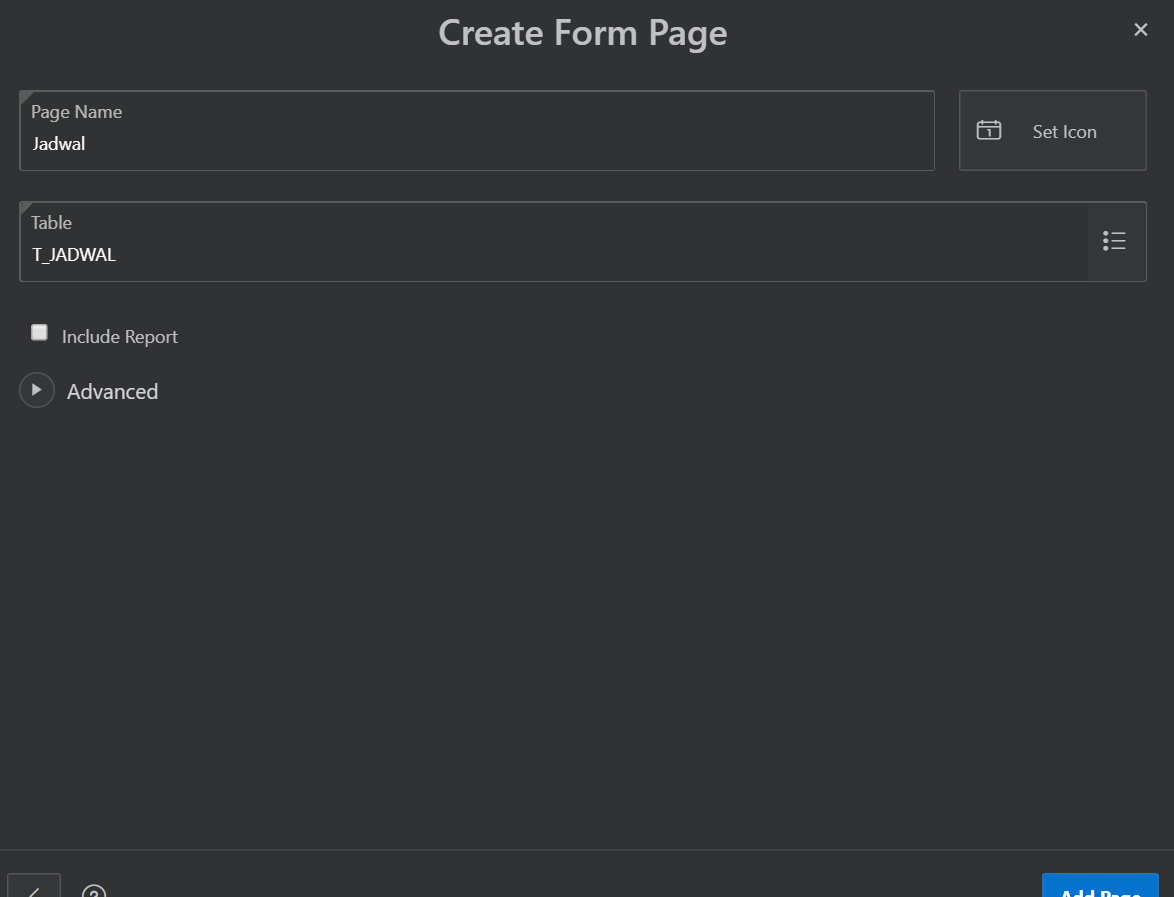
\includegraphics[width=.8\textwidth]{figure/32.PNG}
\end{center}
\begin{center}
    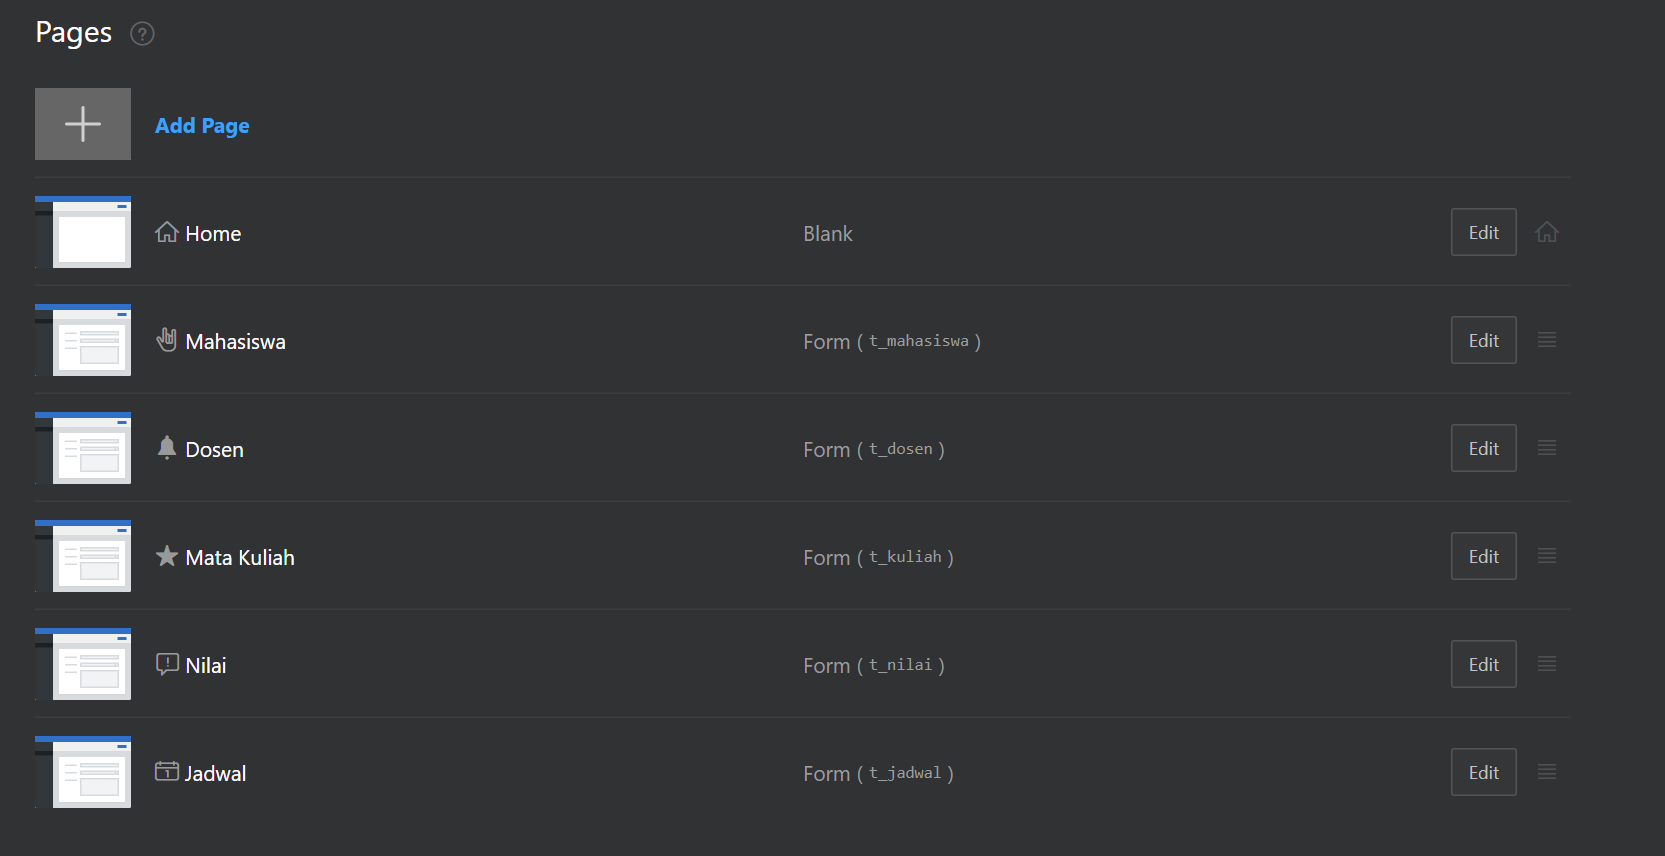
\includegraphics[width=.8\textwidth]{figure/33.PNG}
\end{center}
    \item jika telah selesai scroll kebawa maka akan ada pilihan create application lalu kita klik.
    \begin{center}
    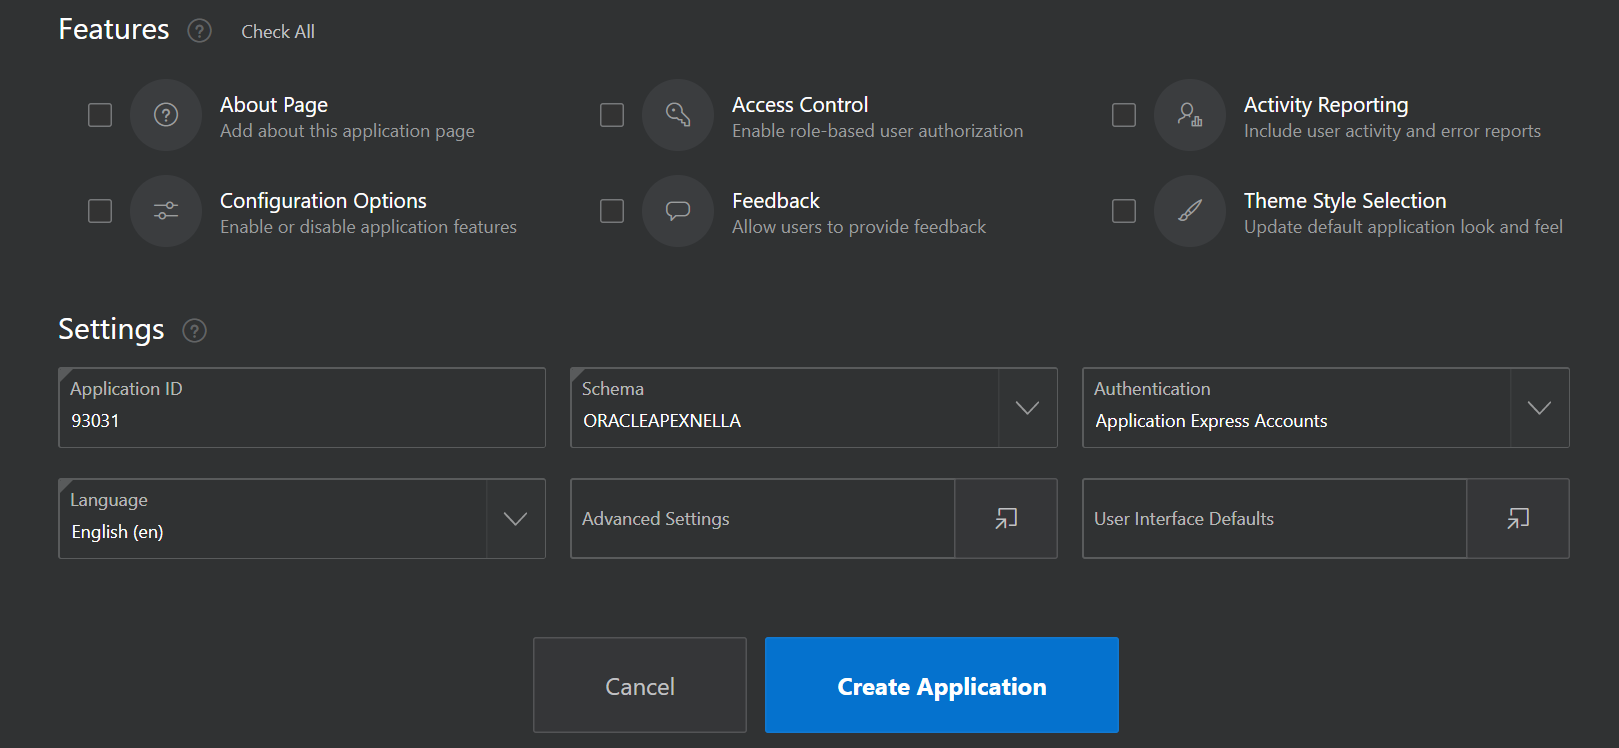
\includegraphics[width=.8\textwidth]{figure/34.PNG}
\end{center}
\begin{center}
    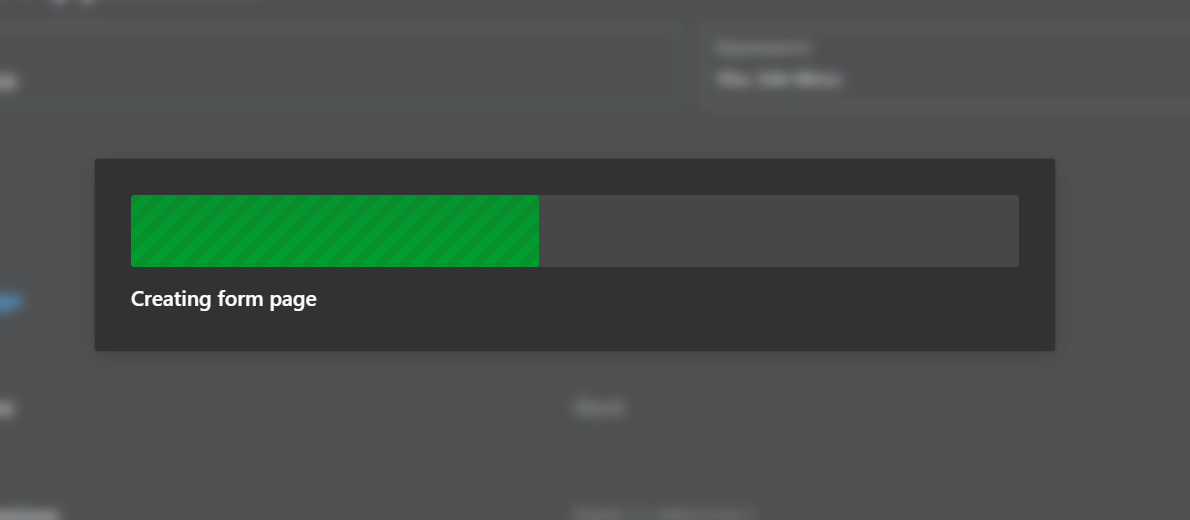
\includegraphics[width=.8\textwidth]{figure/35.PNG}
\end{center}
    \item maka akan tampul menu seperti dibawah ini.dan kita pilih run application ini untuk menjalankan aplikasi.
    \begin{center}
    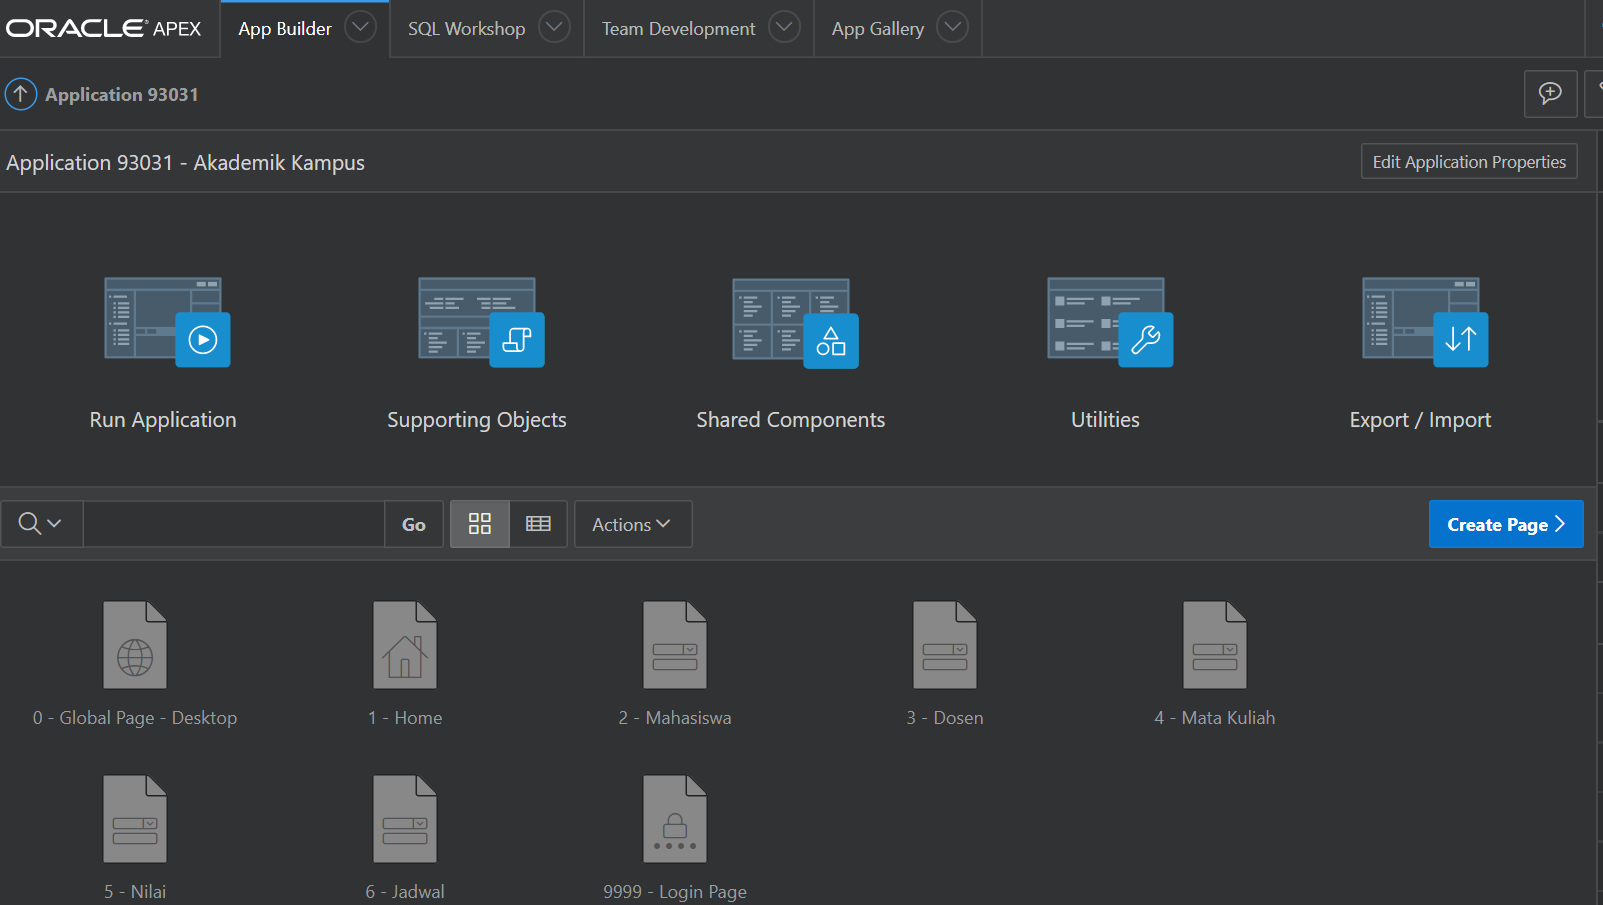
\includegraphics[width=.8\textwidth]{figure/36.PNG}
\end{center}
    \item maka akan muncul form login untuk masuk ke aplikasi.masukkan username dan password.
    \begin{center}
    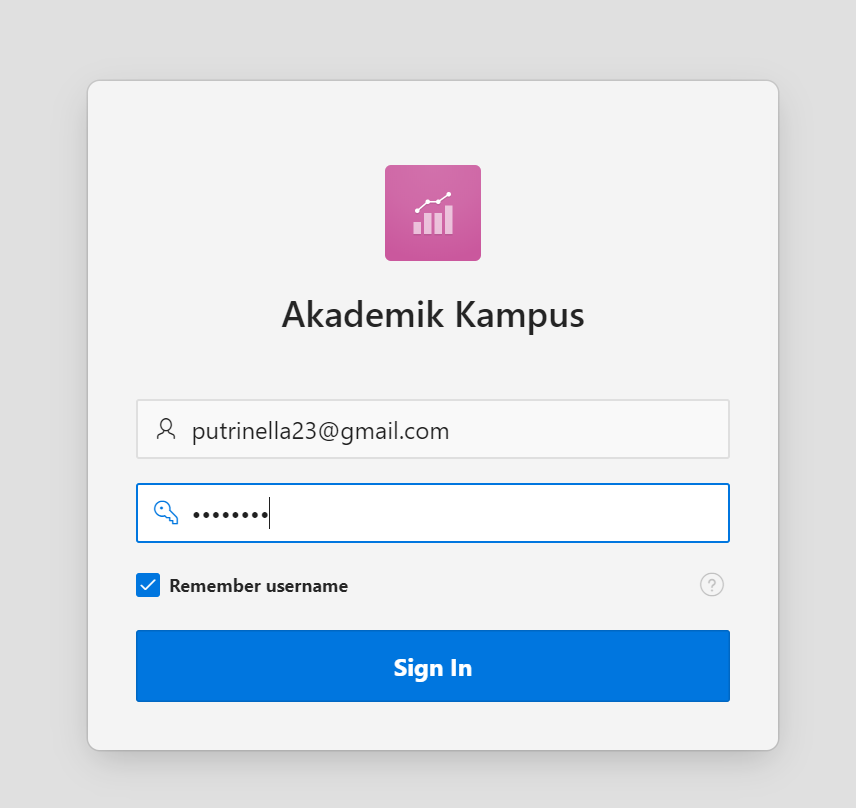
\includegraphics[width=.8\textwidth]{figure/37.PNG}
\end{center}
    \item Setelah masuk,aplikasi yang telah kita buat berhasil.
    \begin{center}
    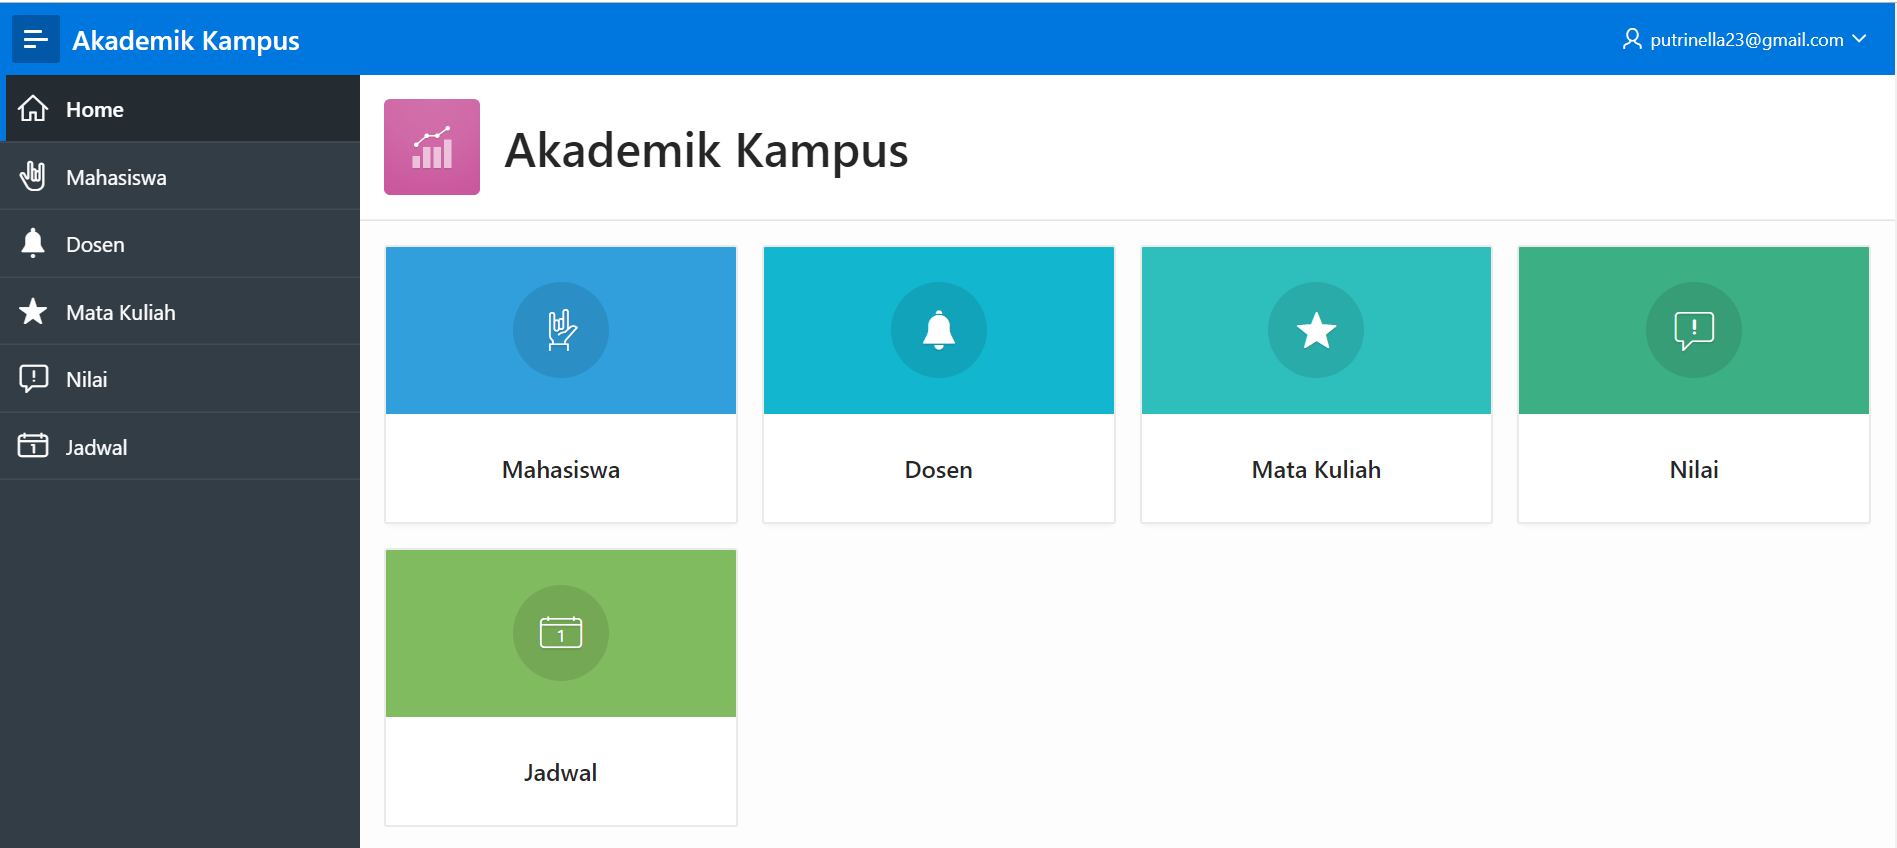
\includegraphics[width=.8\textwidth]{figure/38.PNG}
\end{center}
  
    \item itulah langkah-langkah membuat sistem informasi dengan menggunakan ORACLE APEX.
    \item \usepackage{https://apex.oracle.com/pls/apex/f?p=93031:LOGIN_DESKTOP:700115047311535:::::} 
    \item username :putrinella23@gmail.com\\
          password :nella118
\end{enumerate}
\end{document}
